\chapter{Molecular mechanisms of aspartate limitation}
blaa

\section{Introduction}
More blaa




\section{Mitochondrial inhibition induces a stable relationship between aspartate levels and proliferation rate}
%%% Experiments with H1299 and count/metabolites per day
%% Under ETCinhib_timeseries in lab-work







\section{Quantifying the metabolic fates of aspartate}


\begin{figure}
     \centering
     \begin{subfigure}[b]{0.75\textwidth}
         \centering
         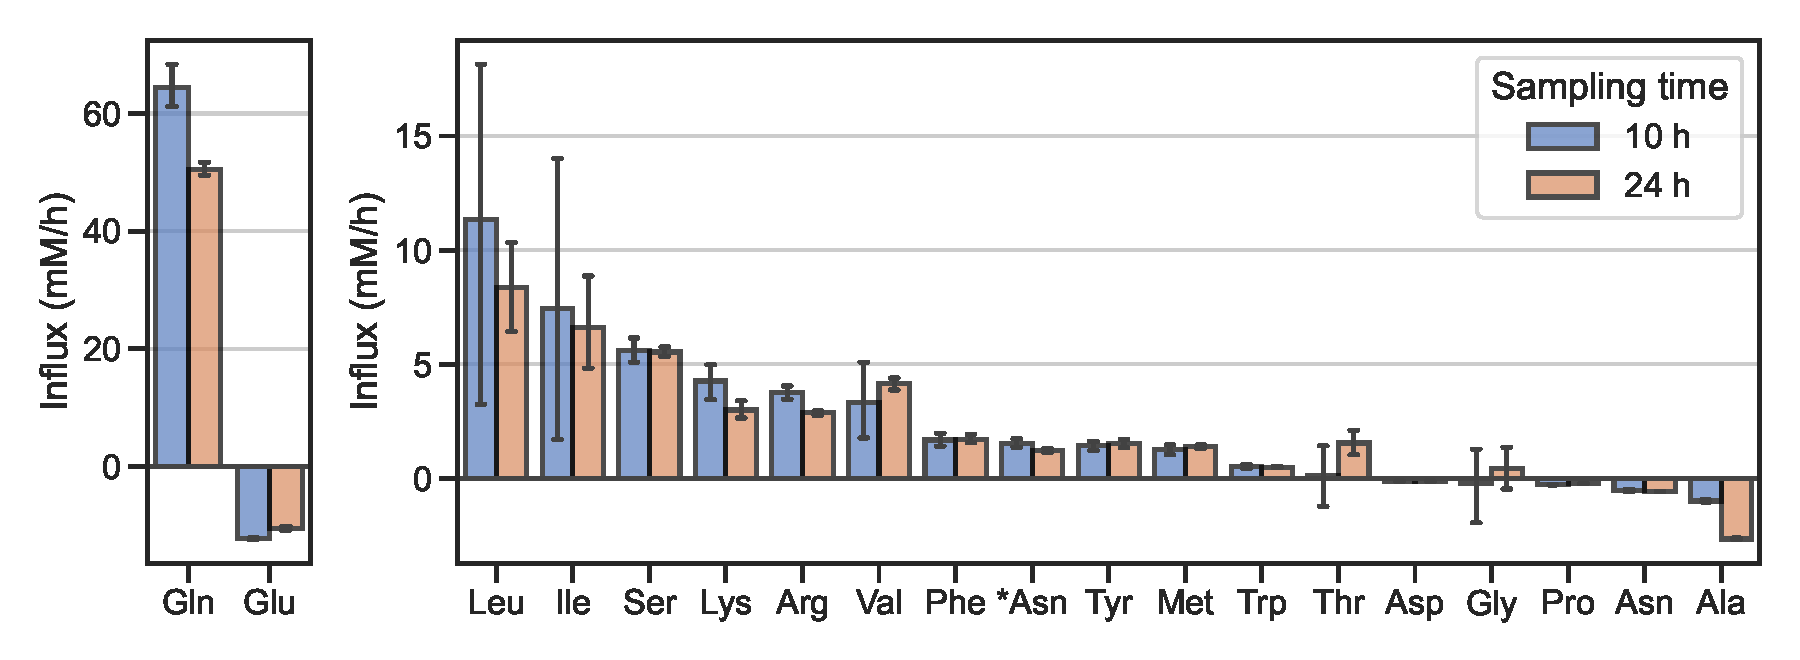
\includegraphics[width=\textwidth]{figures/chap2/flux_143wt.pdf}
         \caption{Media uptake 143B WT}
         \label{fig:ch2:flux_143wt}
     \end{subfigure}
     \begin{subfigure}[b]{0.75\textwidth}
         \centering
         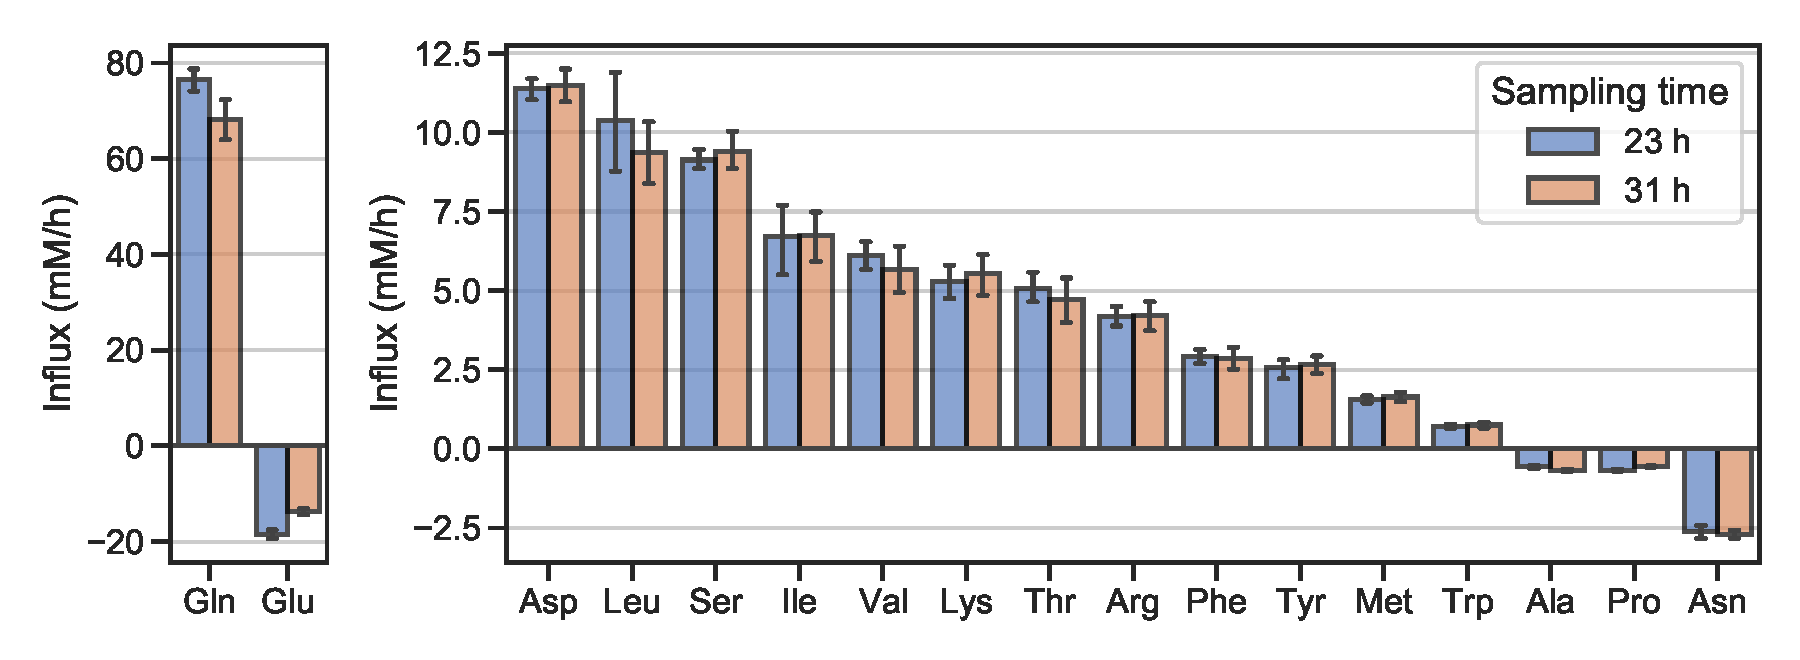
\includegraphics[width=\textwidth]{figures/chap2/flux_143dko.pdf}
         \caption{Media uptake 143B GOT DKO}
         \label{fig:ch2:flux_143dko}
     \end{subfigure}
        \caption[Media amino acid uptake]{
        Amino acid influx/efflux from DMEM.
        For 143B WT in (a), media was spiked with U-\hCi{} Asn (*Asn in the plot) to measure asparagine uptake which, taken together with the labelling fraction, was used to calculate the net asparagine consumption.
        For 143B GOT DKO in (b), cell expressed Glu/Asp transporter SLC1A3 and media was spiked with aspartate to measure its uptake.
        }
\end{figure}



Good correspondence between Asn efflux estimated through labelled Asn in 143B WT (figure \ref{fig:ch2:Asn_flux}) and measured Asn efflux in 143B GOT DKO (figure \ref{fig:ch2:flux_143dko}).
\begin{figure}
     \centering
     \hspace{0.05\textwidth}
     \begin{subfigure}[b]{0.35\textwidth}
         \centering
         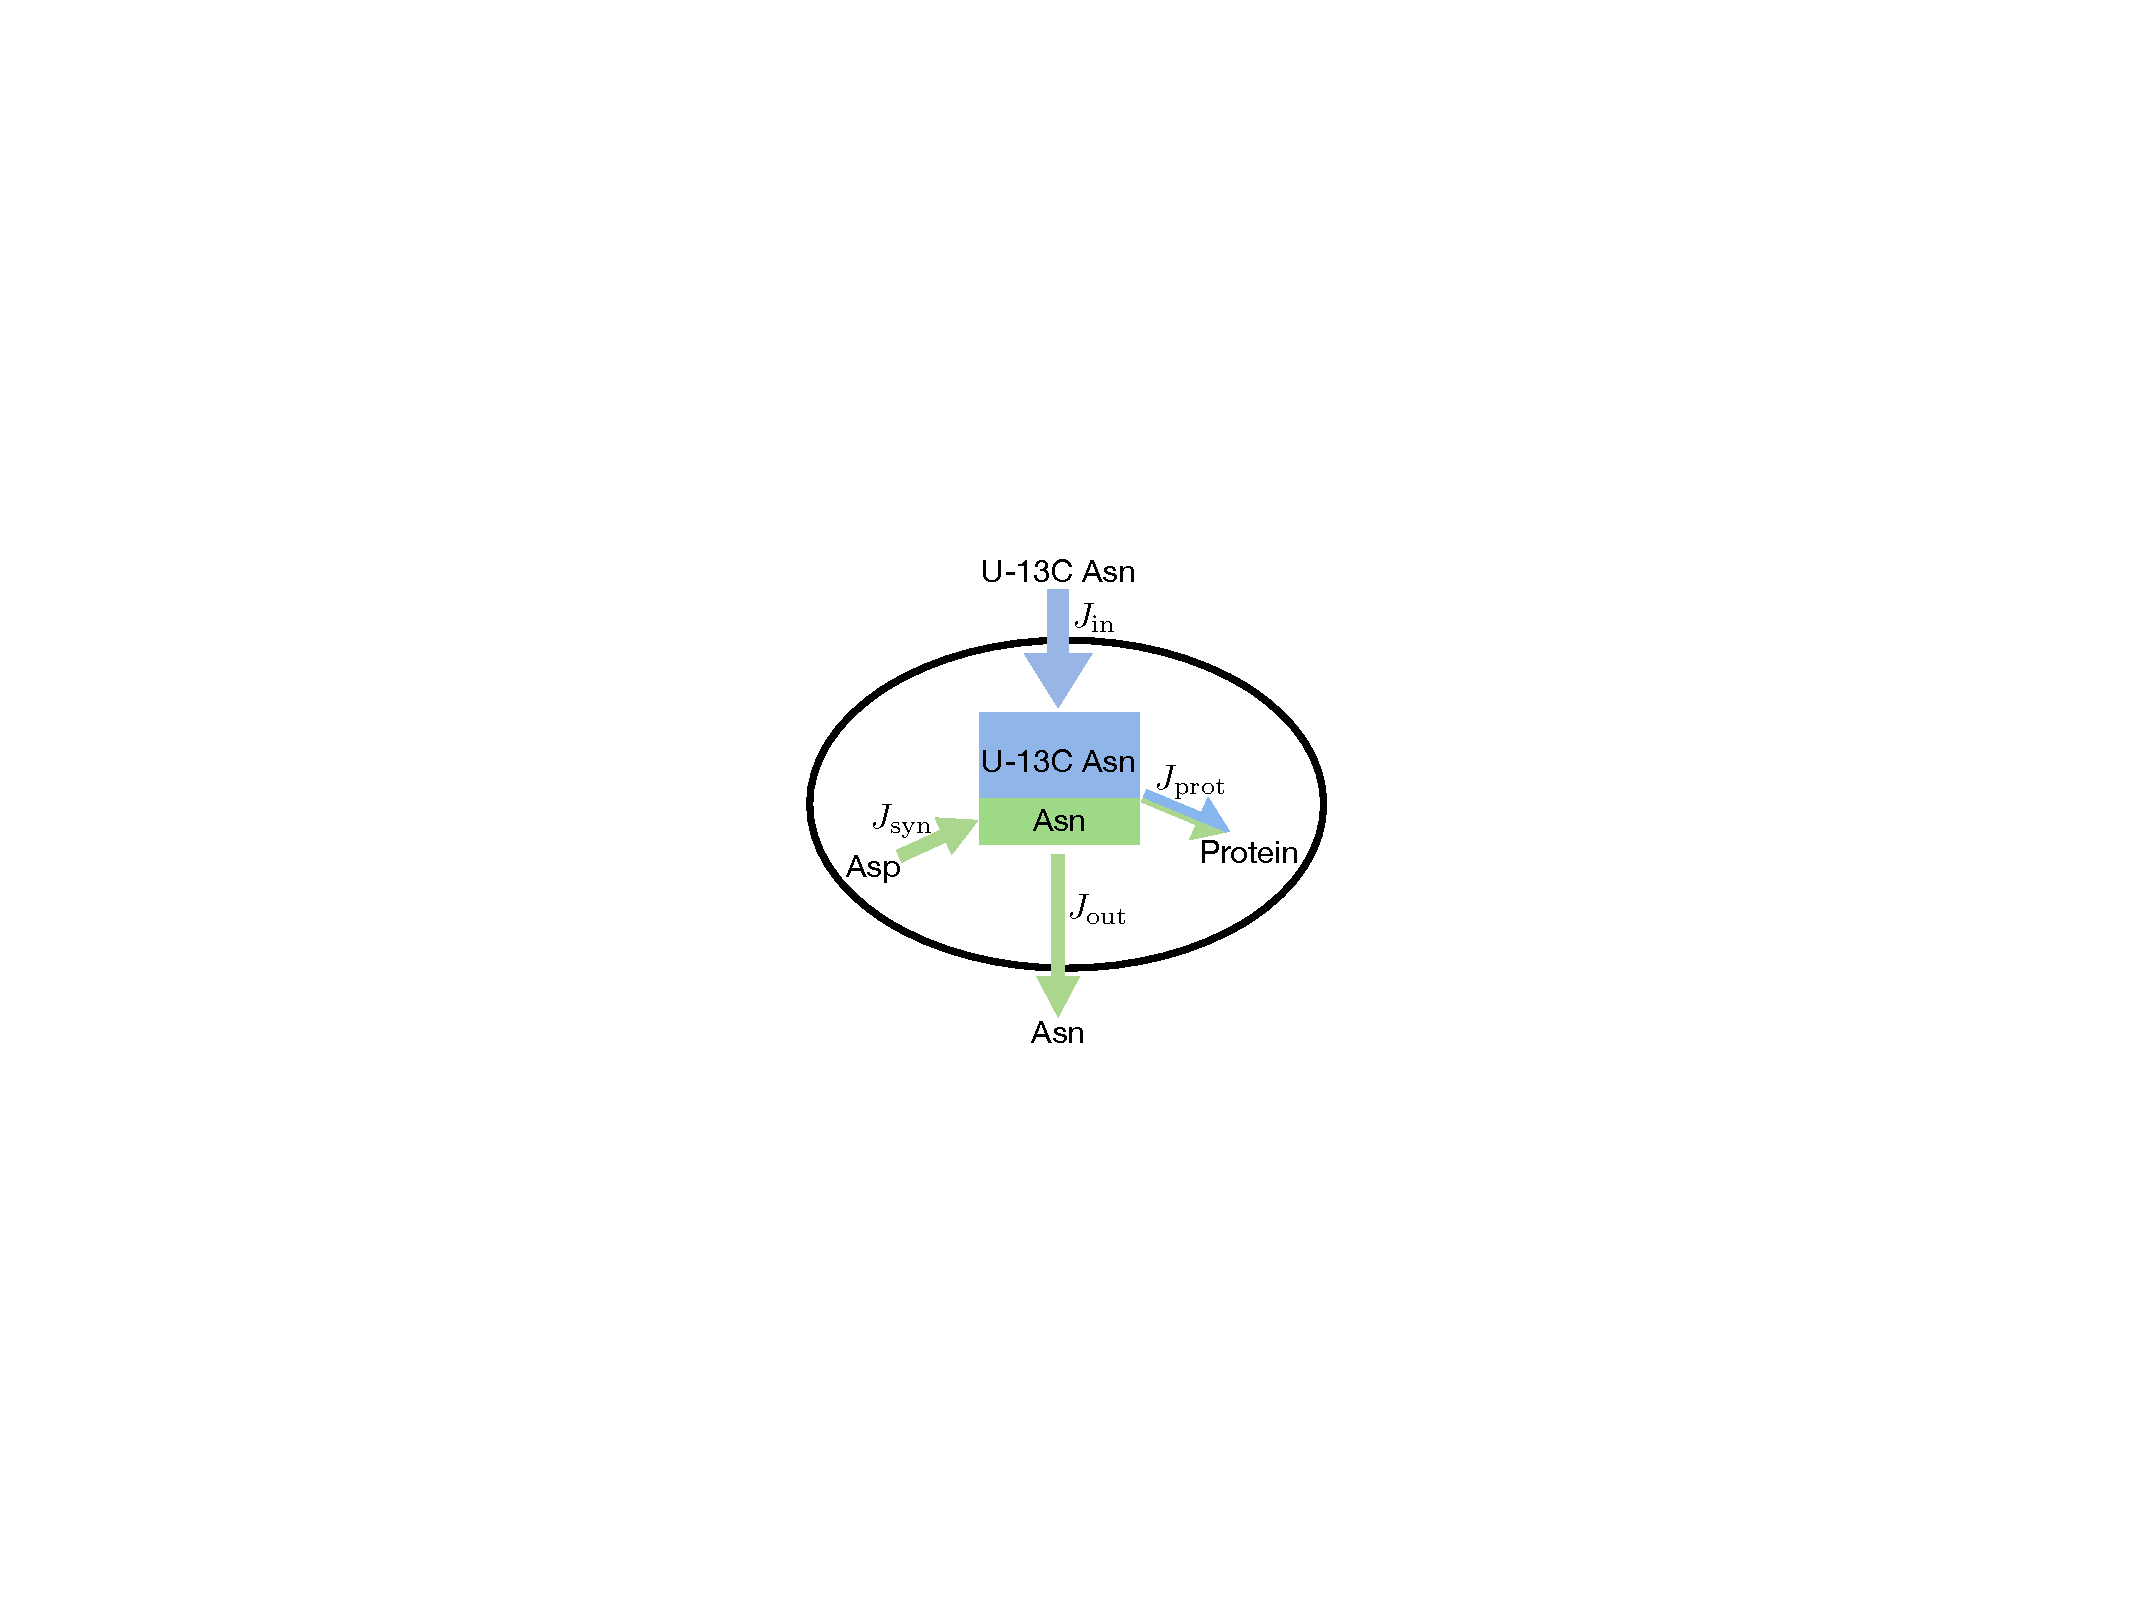
\includegraphics[width=\textwidth]{figures/chap2/asn_Jprot.pdf}
         \caption{Flux diagram}
         \label{fig:ch2:asn_Jprot}
     \end{subfigure}
     \hfill
     \begin{subfigure}[b]{0.4\textwidth}
         \centering
         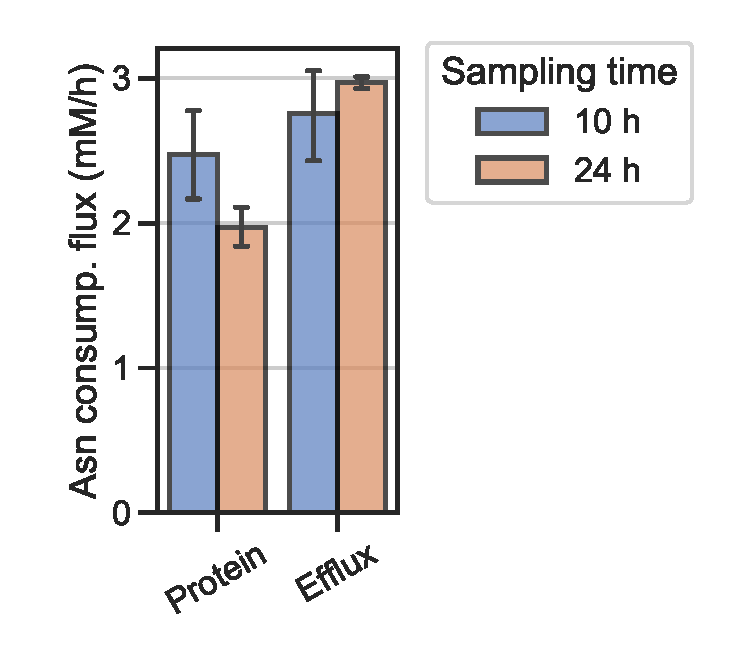
\includegraphics[width=\textwidth]{figures/chap2/Asn_flux.pdf}
         \caption{Asn consumption}
         \label{fig:ch2:Asn_flux}
     \end{subfigure}
     \hspace{0.05\textwidth}
        \caption[Asparagine consumption fluxes]{
        (a) Diagram of asparagine fluxes in a cell.
        Net influx of U-\hCi{} labelled Asn ($\Flin$), net efflux of unlabelled Asn ($\Flout$), net deposition of Asn into protein ($\Flprot$) and Asn synthesis from Asp ($\Flsyn$).
        Asn symbolized by green and U-\hCi{} Asn symbolized by blue.
        (b) Measured asparagine consumption fluxes in 143B cells using the media uptake data from figure \ref{fig:ch2:flux_143wt}.
        Asn is consumed into protein synthesis (Protein) and leaked into the media (Efflux).
        Efflux is calculated assuming no Asn is provided in the media.
        }
\end{figure}



Most of cellular biomass is amino acids \cite{Hosios2016-us}

\begin{figure}
    \centering
    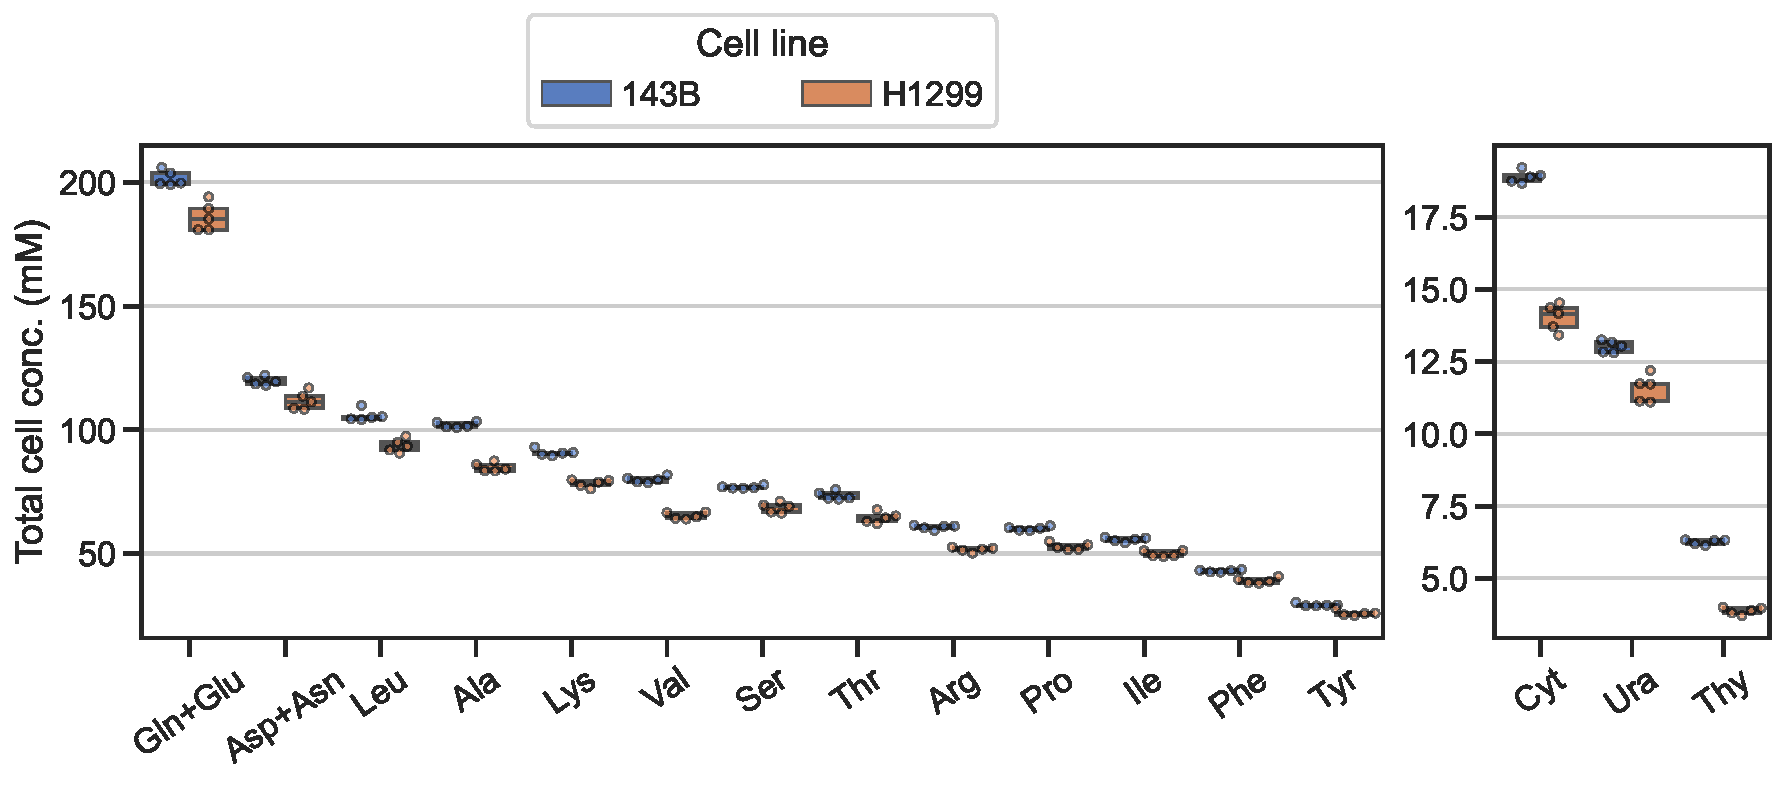
\includegraphics[width=0.80\textwidth]{figures/chap2/ah_cell_comp.pdf}
    \caption[Amino acid and pyrimidine total cell concentration]{
    Total amino acids and pyrimidines liberated by acid hydrolysis of 143B and H1299 cells, normalized by total cell volume (Total cell conc.).
    Gln and Asn is converted during acid hydrolysis to Glu and Asp respectively.
    }
    \label{fig:ch2:ah_cell_comp}
\end{figure}






The total Asp consumption flux expected in DMEM i.e. with Arg but without Asn, is estimated to be 9.25 mM/h.
This is close to Asp uptake in 143B GOT DKO which was measured at 11.43 mM/h (figure \ref{fig:ch2:flux_143dko}).
The difference is directionally as would be expected because total pyrimidine/purine levels underestimate synthesis flux by discounting recycling (figure ]\ref{fig:ch2:pur_tr_ov}) and because 143B GOT DKO maintain a higher intracellular concentration of aspartate due to expression of Glu/Asp transporter SLC1A3.
\begin{figure}
    \centering
    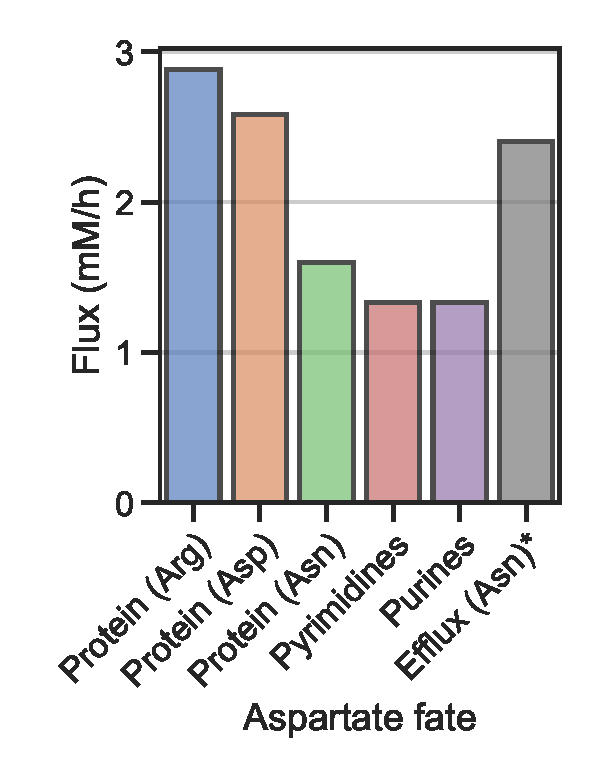
\includegraphics[width=0.36\textwidth]{figures/chap2/asp_fate.pdf}
    \caption[Relative consumption towards each fate of aspartate]{
    Relative consumption towards each fate of aspartate estimated using best estimates from figure \ref{fig:ch2:Asn_flux} and \ref{fig:ch2:ah_cell_comp}.
    Aspartate consumption towards purines was estimated equal to consumption towards pyrimidines.
    * Asn efflux is calculated based on the assumption that cells are grown in asparagine free media, prior to substantial media conditioning.
    }
    \label{fig:ch2:asp_fate}
\end{figure}






\section{Salvage of the metabolic fates of aspartate}

\subsection{Salvage mix fulfills all the metabolic fates of aspartate}

metabolic fates of aspartate i.e. aspartate conversion 


\begin{figure}
    \centering
    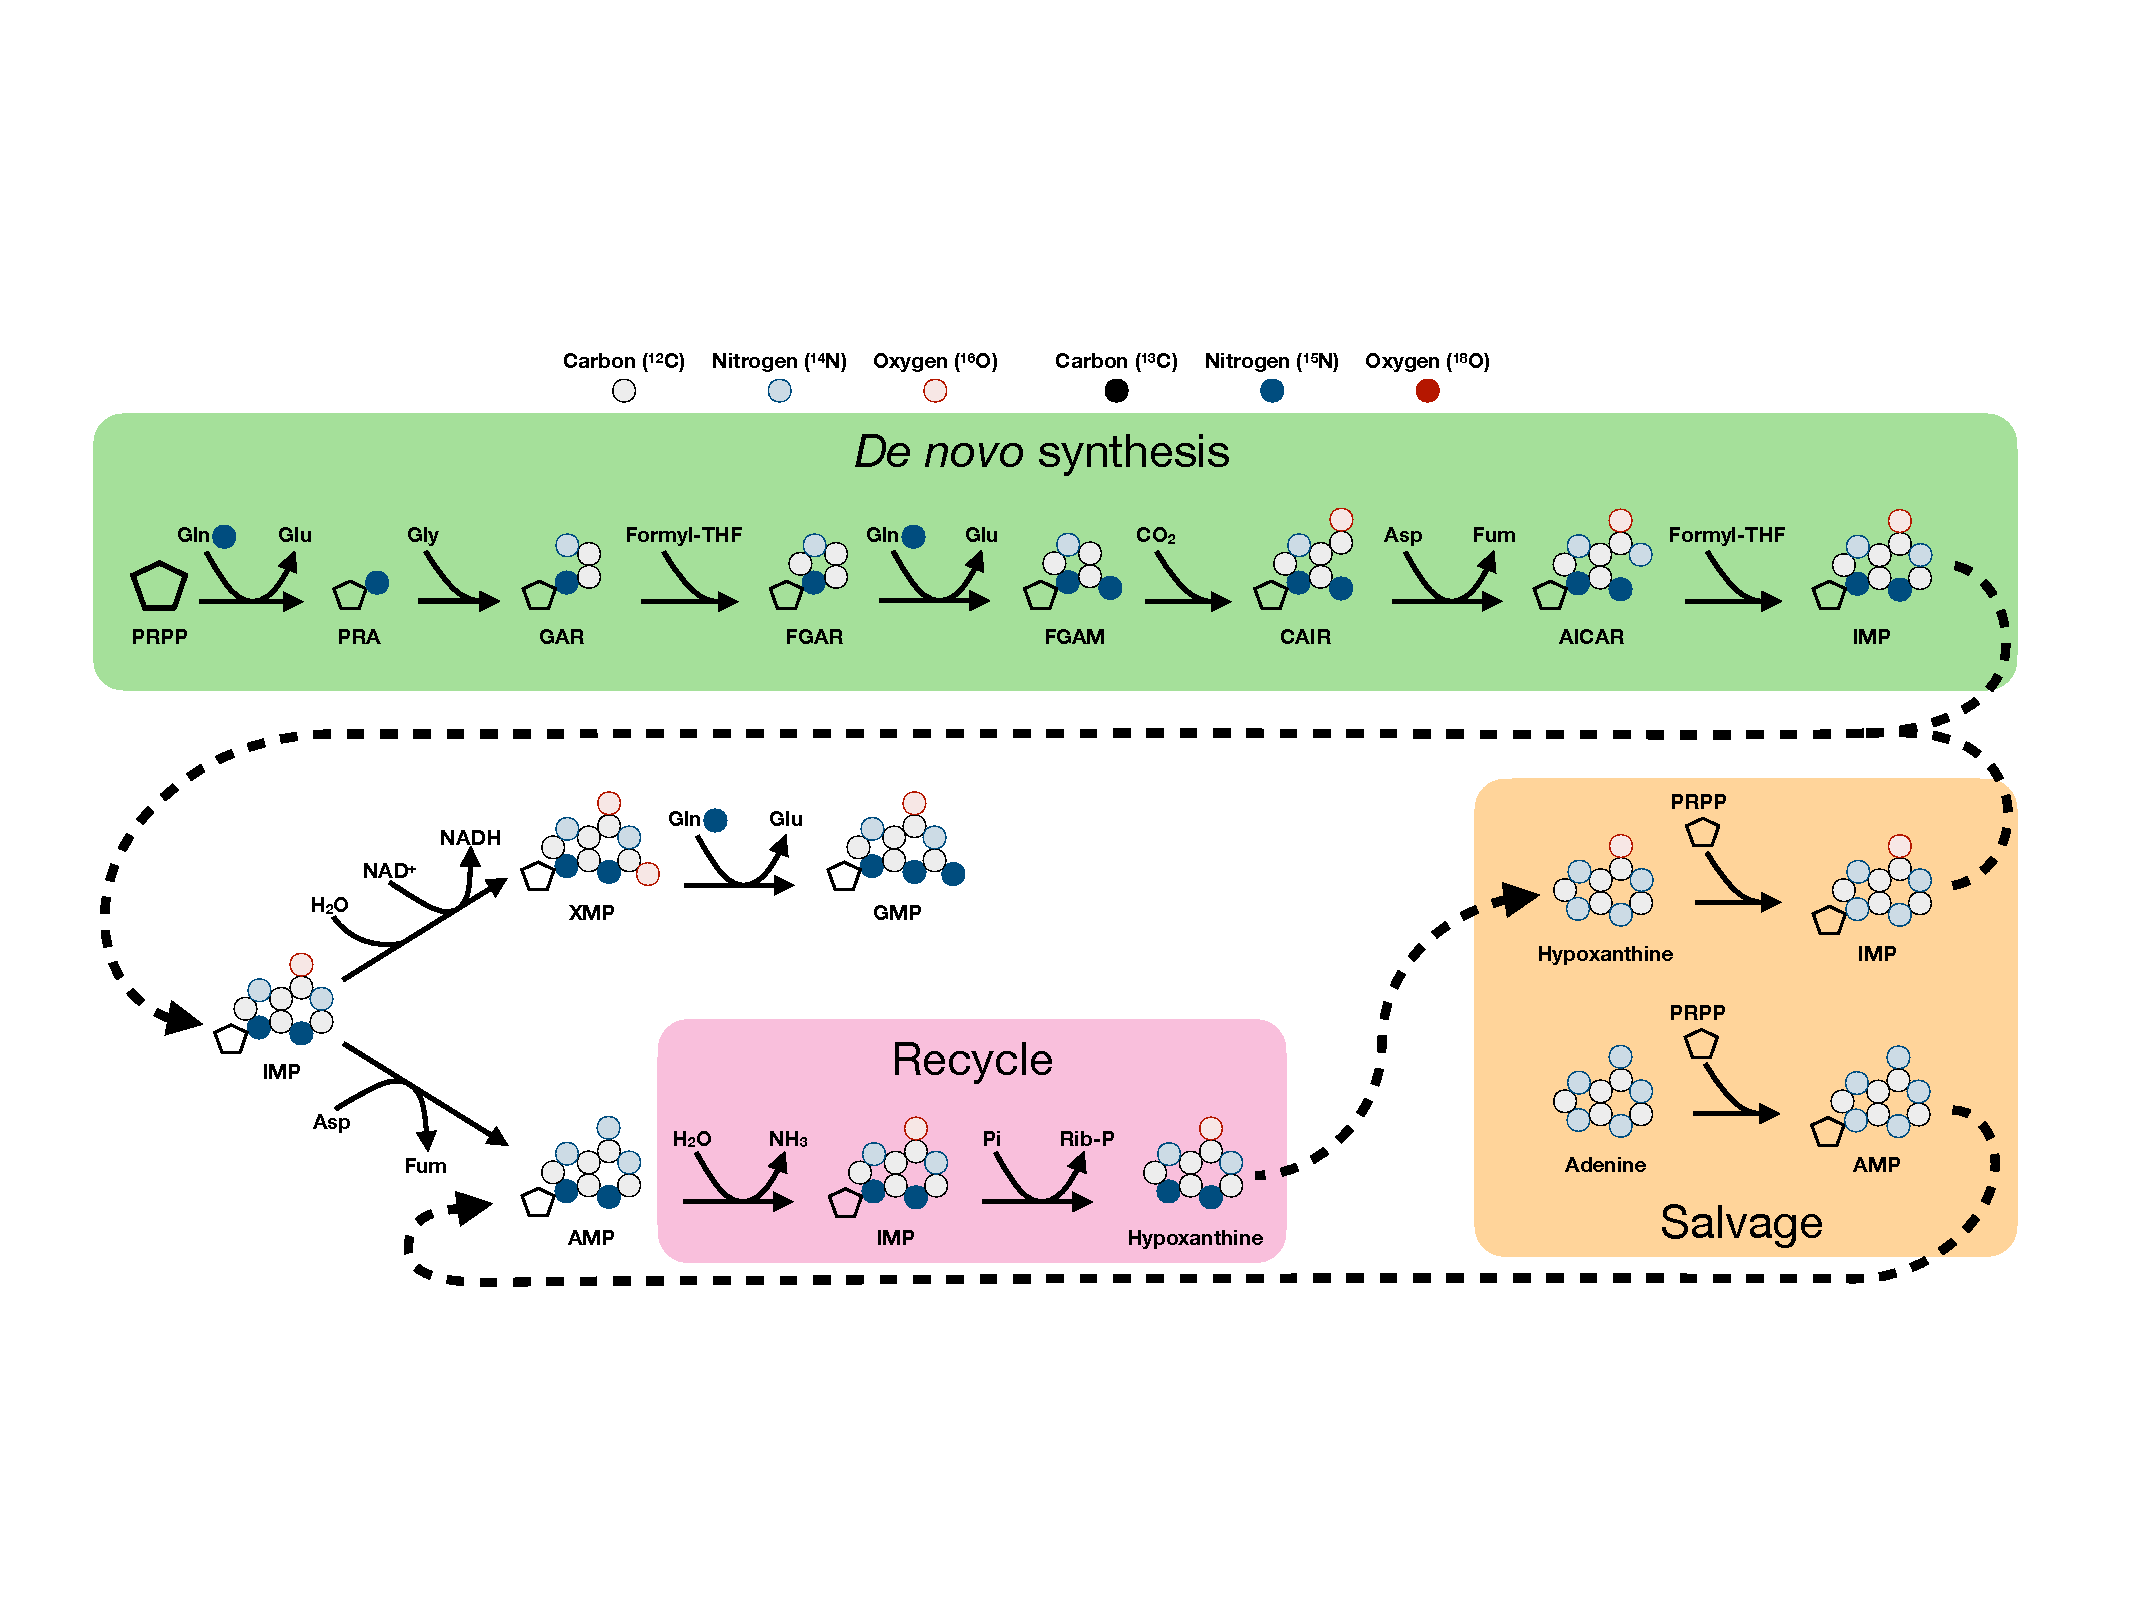
\includegraphics[width=0.95\textwidth]{figures/chap2/purine_tracing_overvew.pdf}
    \caption[Purine metabolism \hNi-amide Gln tracing overview]{
    Overview of \hNi-amide Gln label incorporation in \textit{de novo} purine synthesis.
    Label incorporation can be effected by salvage of unlabelled hypoxanthine or adenine and recycling as it appears on the overview.
    }
    \label{fig:ch2:pur_tr_ov}
\end{figure}





\begin{figure}
    \centering
    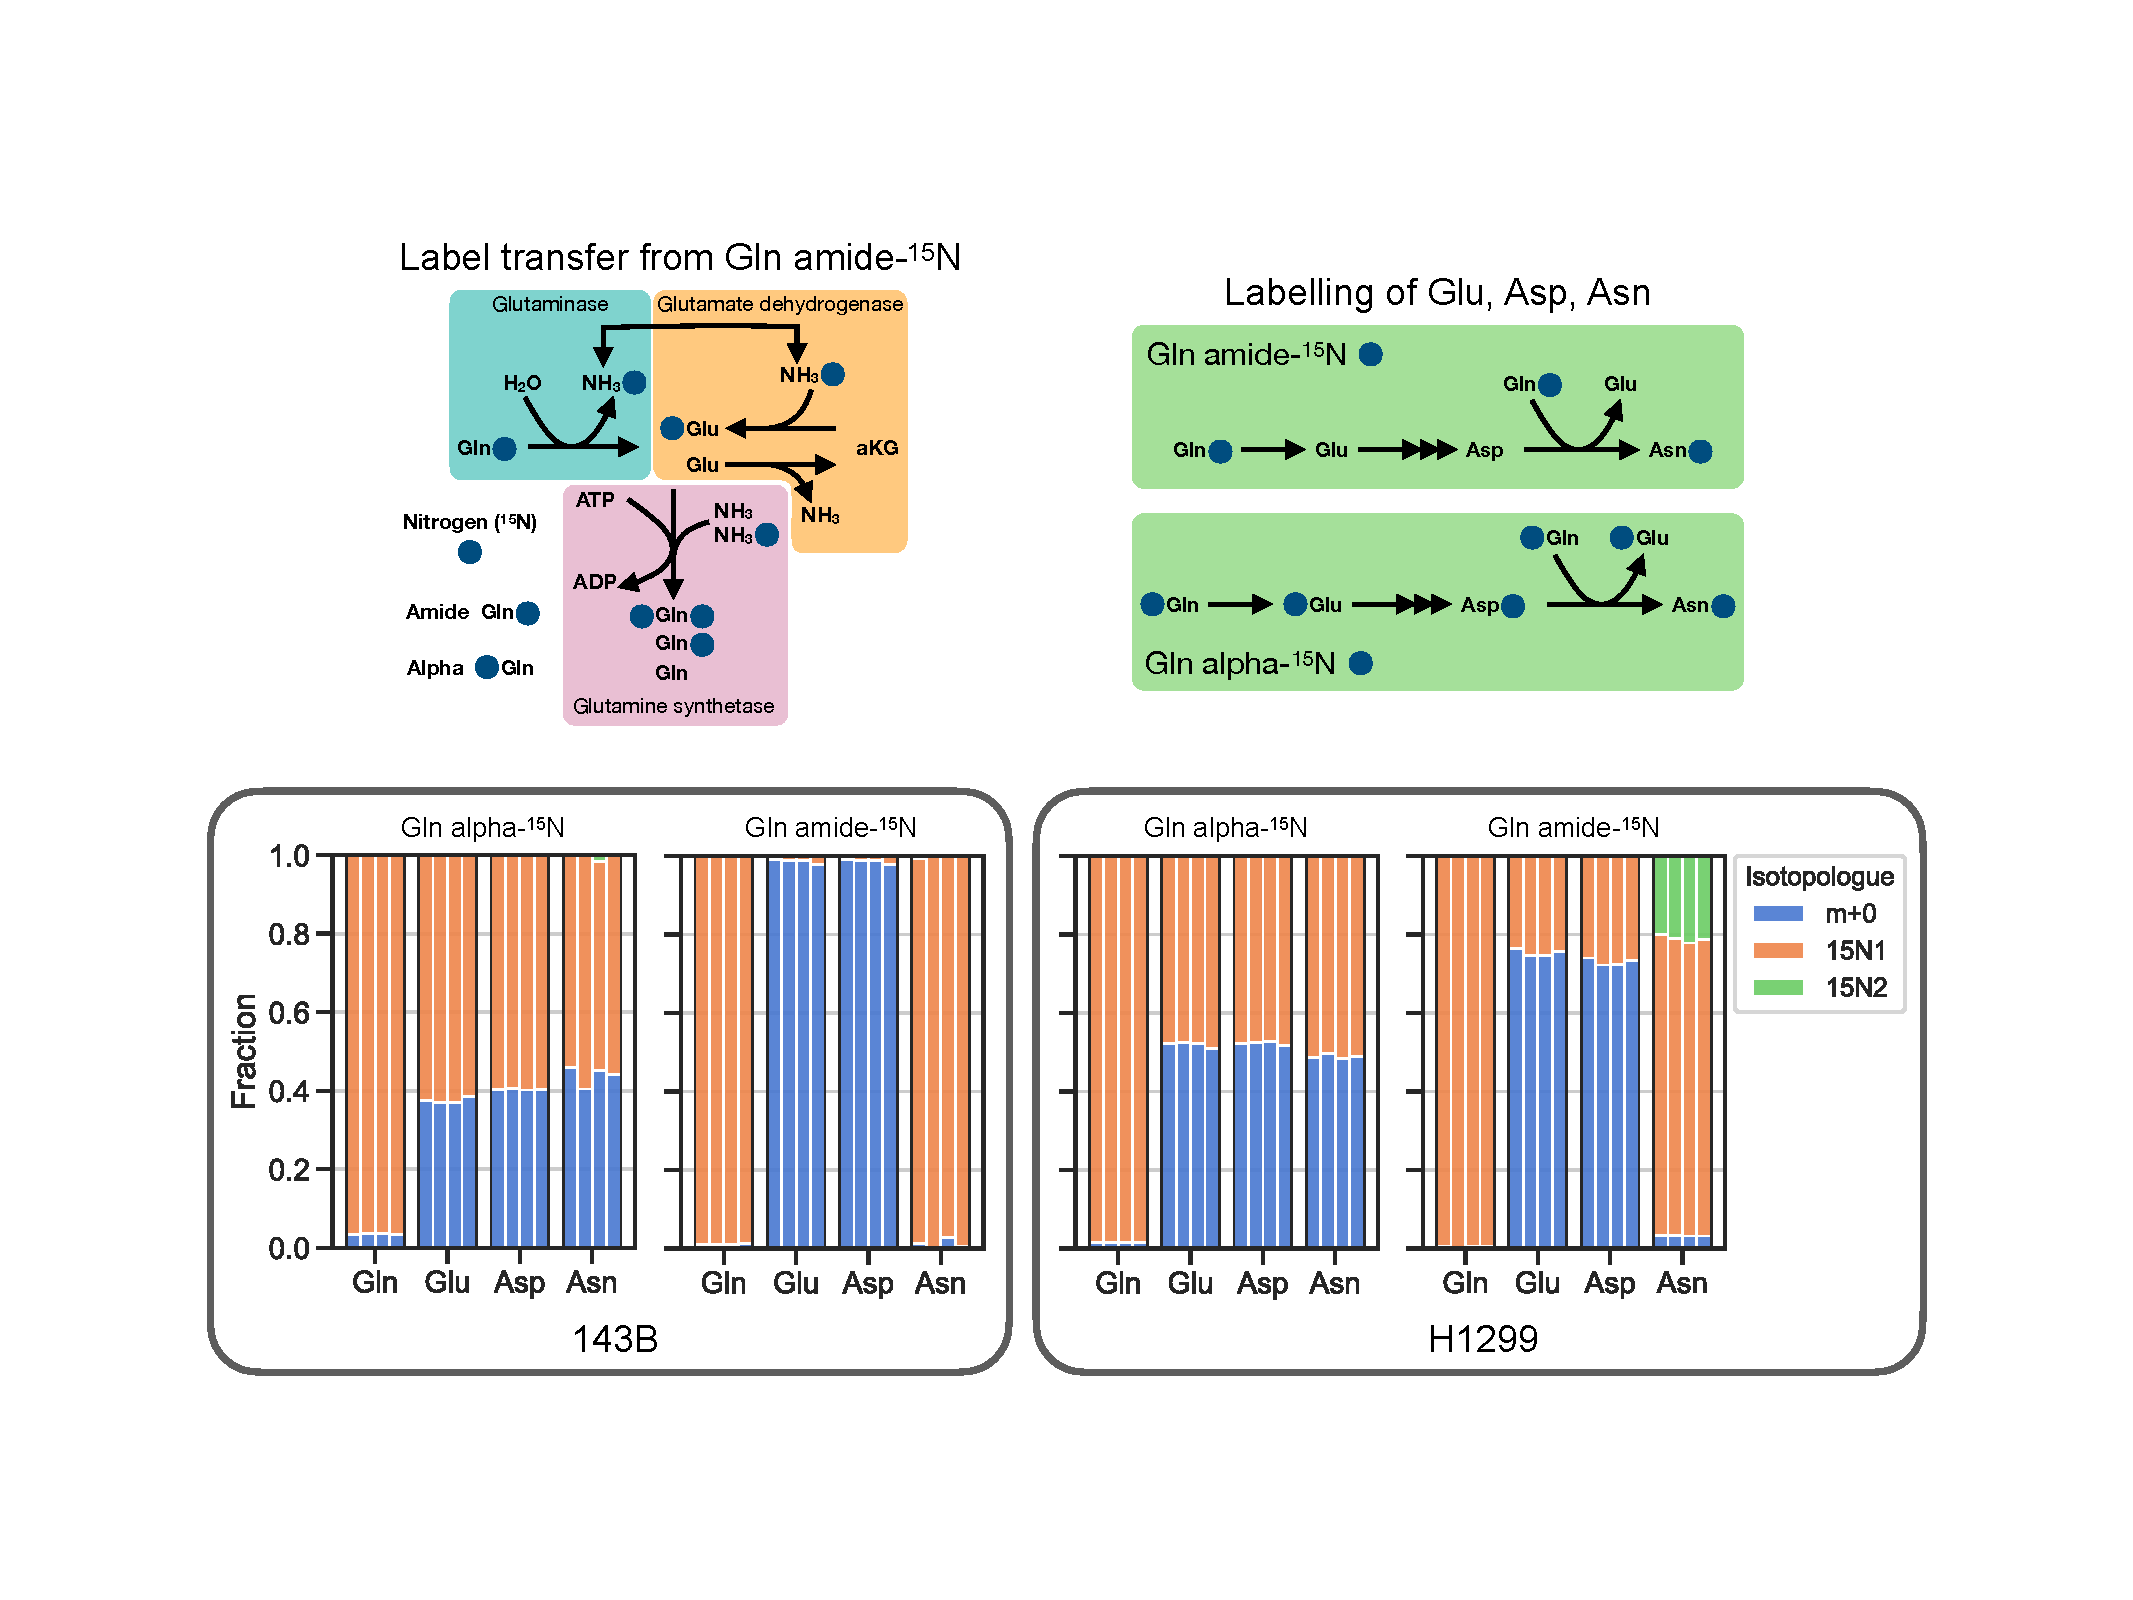
\includegraphics[width=0.95\textwidth]{figures/chap2/gln_lab_tranfr.pdf}
    \caption[Gln amide to alpha \hNi{} transfer]{
    Gln \hNi{} on the amide nitrogen can transfer to the alpha nitrogen in H1299 cells but not in 143B cells.
    Upper left diagram shows how Gln amide and alpha nitrogen labels can transfer.
    Transfer of amide labelled nitrogen can be achieved by glutaminase catalyzed release of labelled ammonia and its subsequent use as a substrate in the conversion of alpha-ketoglutarate (aKG) to Glu alpha-\hNi by glutamate dehydrogenase.
    The signature of glutamine synthetase activity is the appearance of doubly labelled Gln.
    Upper right diagram shows how Gln amide and alpha nitrogen labels are transferred to downstream metabolites Glu, Asp and Asn.
    Lower panel shows the nitrogen isotopologue distribution of Gln, Glu, Asp and Asn in 143B and H1299 at steady-state.
    The alpha nitrogen label is frequently lost in Glu and downstream, presumably due to transaminase catalyzed exchange with unlabelled amino groups on amino acids such as leucine, isoleucine, valine etc.
    The amide nitrogen label is partially transferred to the alpha position in H1299, but not in 143B, also indicated by the doubly labelled Asn.
    }
    \label{fig:ch2:gln_lab_tranfr}
\end{figure}


\begin{figure}
    \centering
    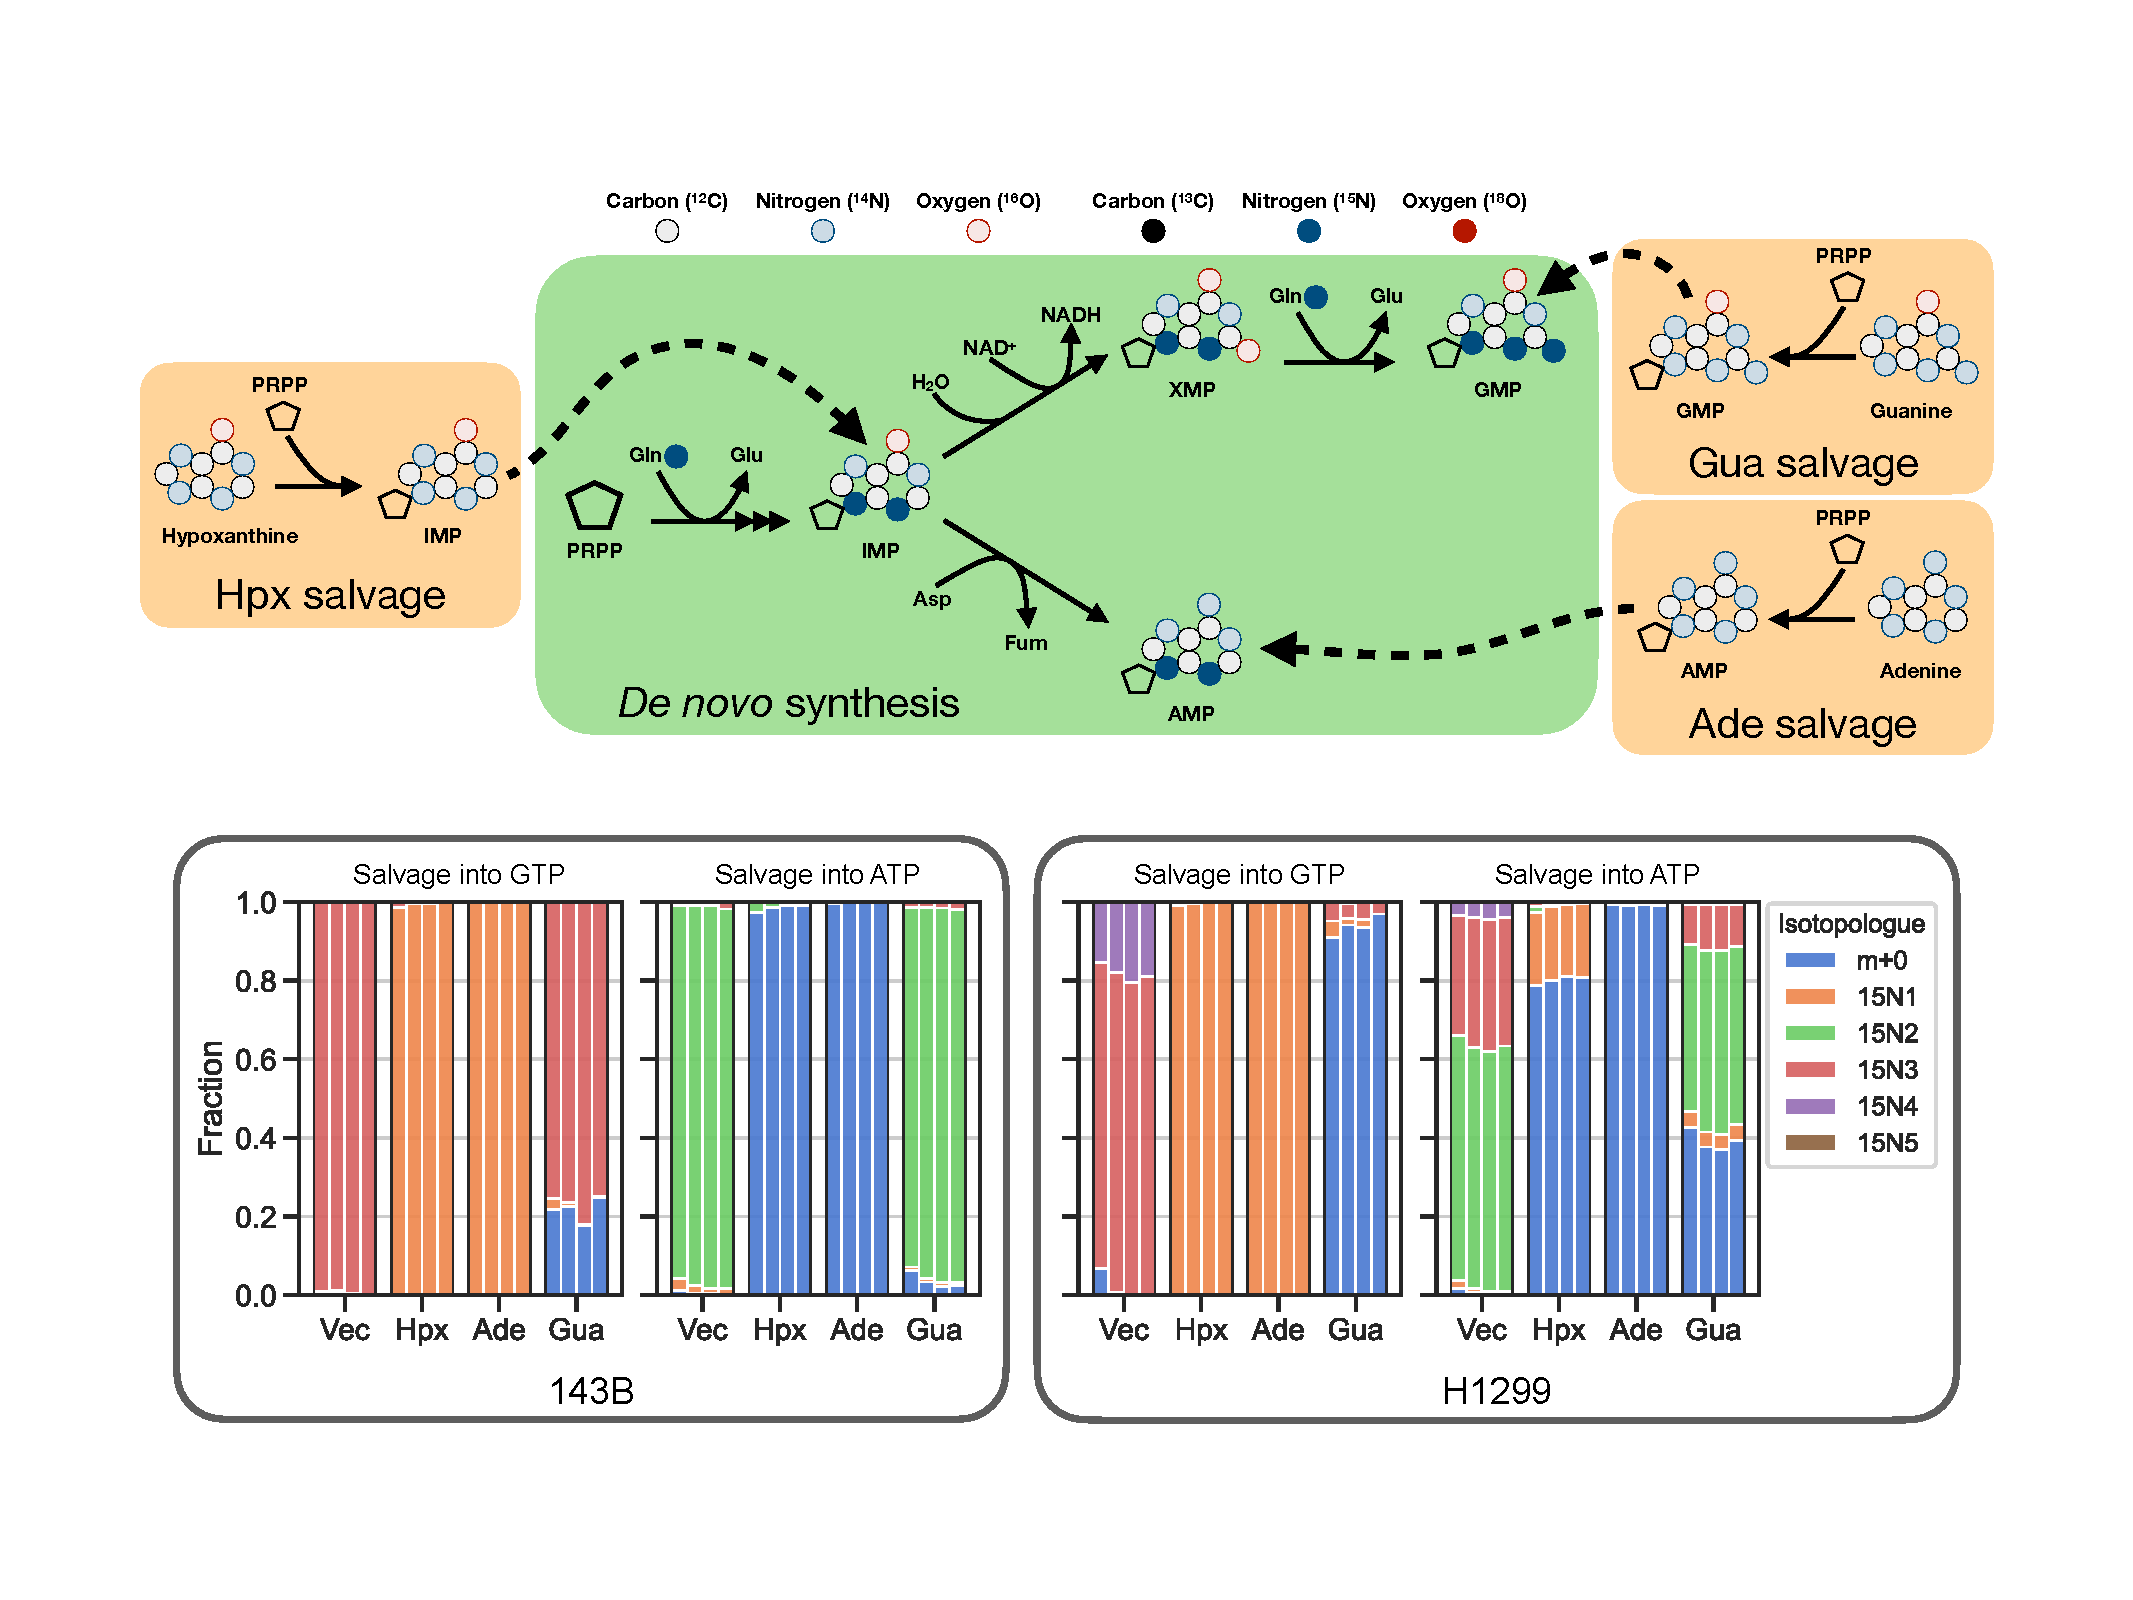
\includegraphics[width=0.98\textwidth]{figures/chap2/sal_frac_pur.pdf}
    \caption[Salvage into purines]{
    ggg
    }
    \label{fig:ch2:sal_frac_pur}
\end{figure}


\begin{figure}
    \centering
    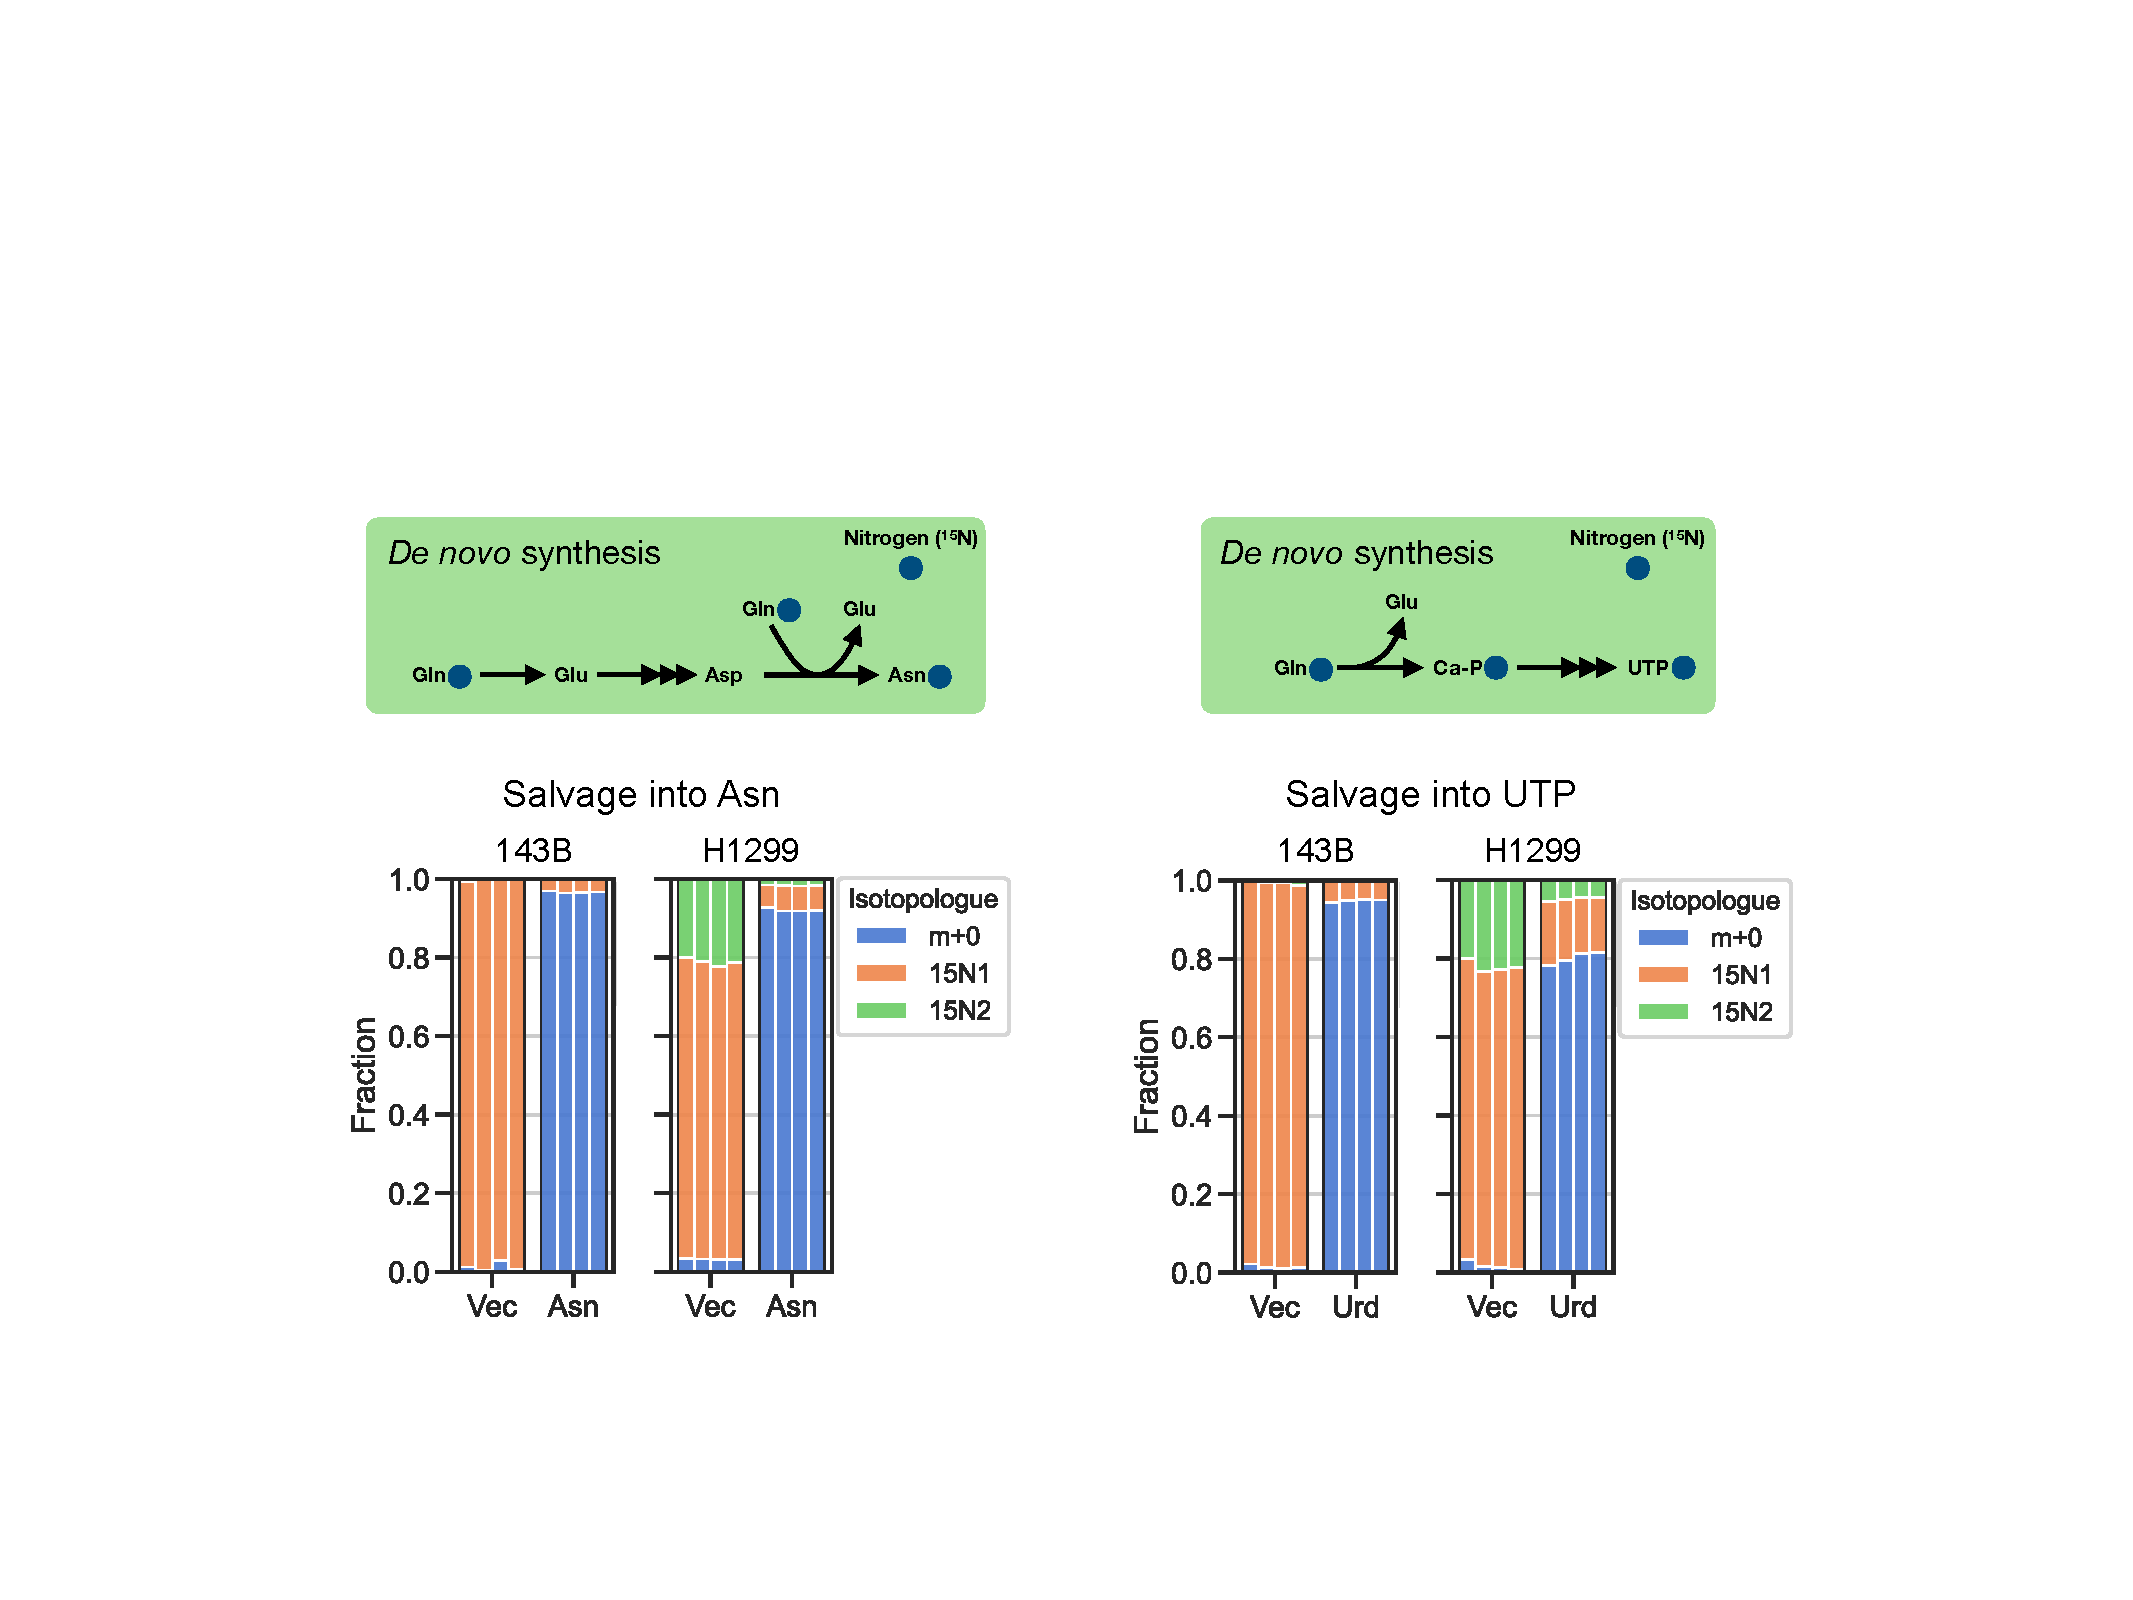
\includegraphics[width=0.8\textwidth]{figures/chap2/sal_frac_pyr-asn.pdf}
    \caption[Salvage into asparagine and pyrimidines]{
    ggg
    }
    \label{fig:ch2:sal_frac_pyr-asn}
\end{figure}









\begin{figure}
    \centering
    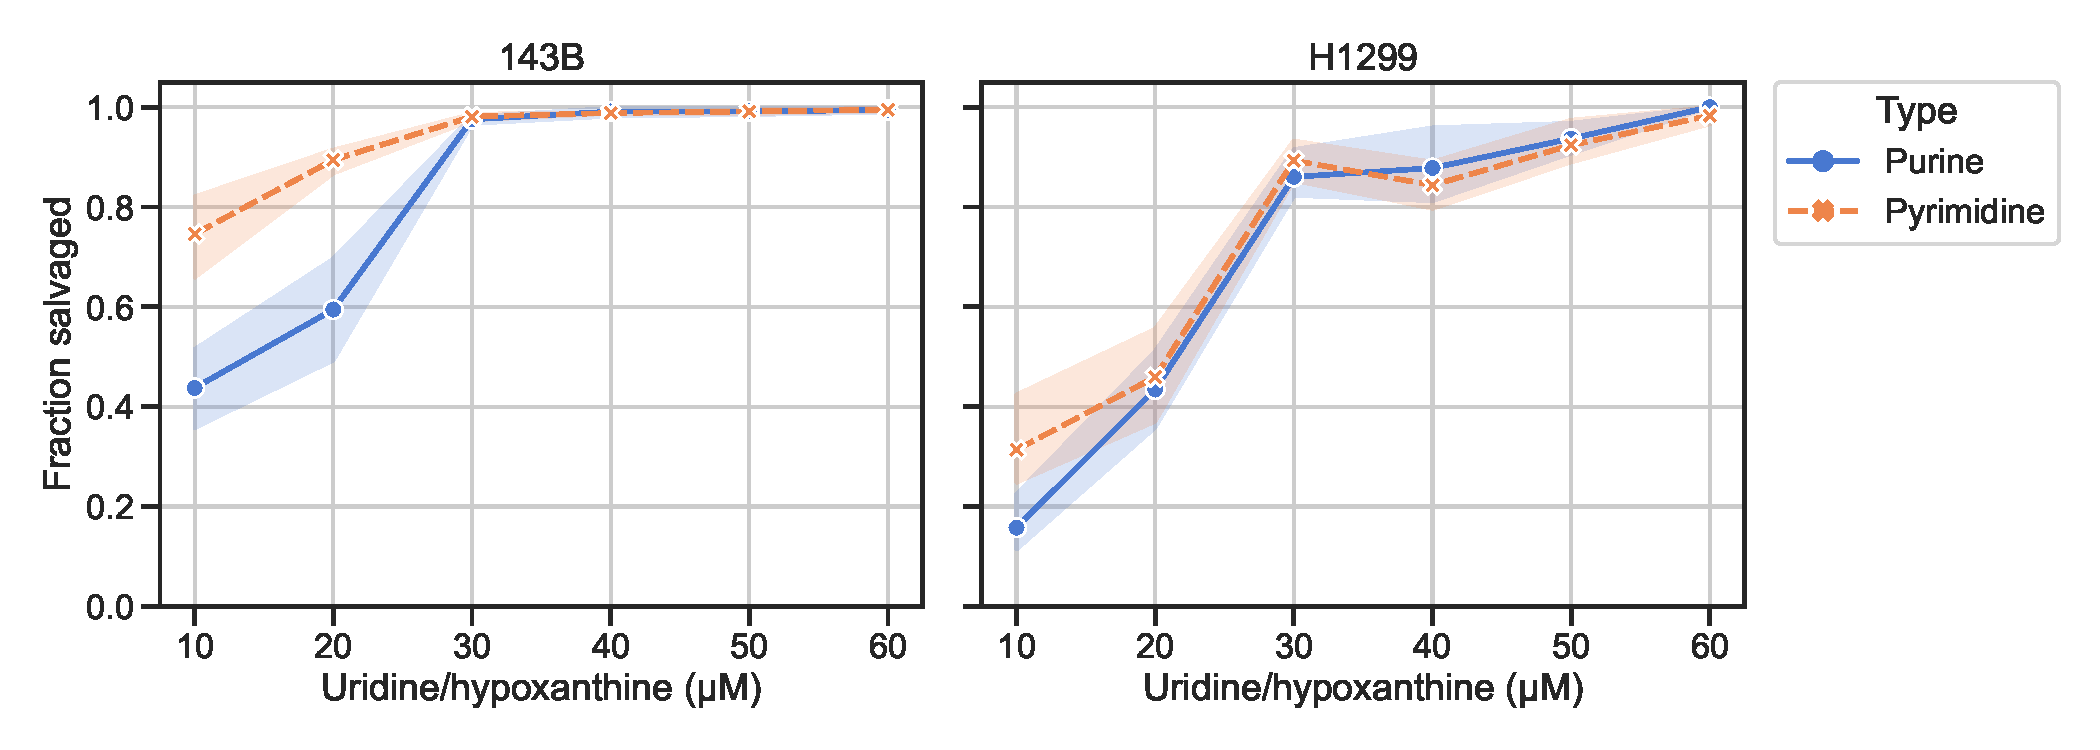
\includegraphics[width=0.95\textwidth]{figures/chap2/sal_frac_conc.pdf}
    \caption[Salvage as a function of Urd/Hpx concentration]{
    Fraction of purines (GDP, GMP, ADP and AMP) and pyrimidines (UDP, UMP, CDP and CMP) derived from salvage when 143B or H1299 cells are cultured in increasing concentrations of uridine/hypoxanthine.
    }
    \label{fig:ch2:sal_frac_conc}
\end{figure}







\section{Aspartate to proliferation curves}

%%% Experiments with individual components under "ETCrescue" folder in lab-work

%%% Experiments with H1299 (Metformin and Rotenone) and HT1080




\section{Integrated stress response}

Overlap between perturbations eliciting ISR by GCN2 and HRI \cite{Taniuchi2016-nc}



\begin{figure}
     \centering
     \begin{subfigure}[b]{0.49\textwidth}
         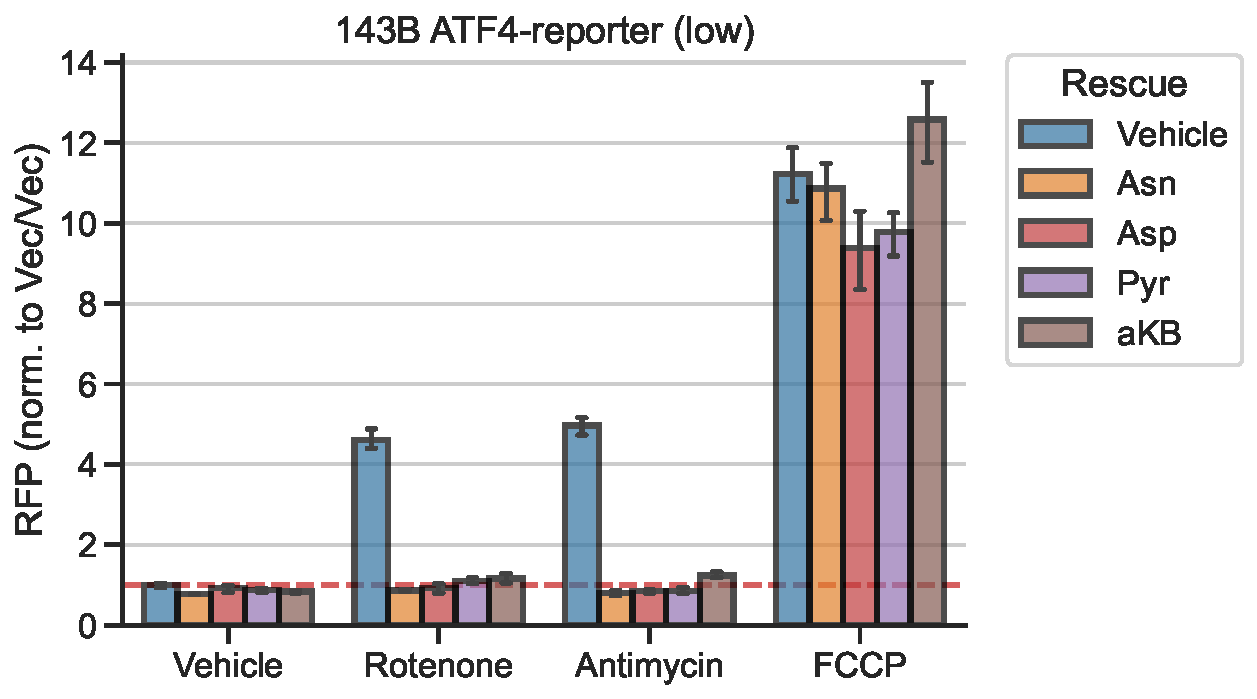
\includegraphics[width=\textwidth]{figures/chap2/143B_ETCinhib_ATF4rep_low.pdf}
         \caption{ggg}
         \label{fig:ch2:143B_ETCinhib_ATF4rep_low}
     \end{subfigure}
     \hfill
     \begin{subfigure}[b]{0.49\textwidth}
         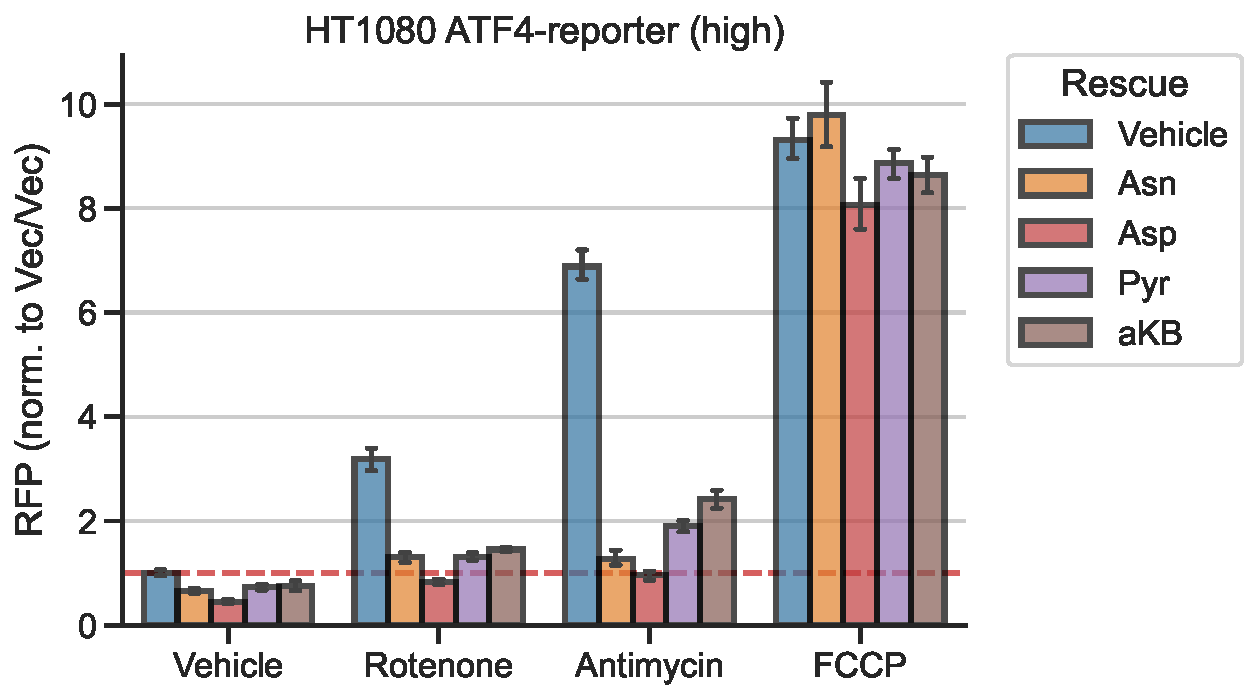
\includegraphics[width=\textwidth]{figures/chap2/HT1080_ETCinhib_ATF4rep_high.pdf}
         \caption{ggg}
         \label{fig:ch2:HT1080_ETCinhib_ATF4rep_high}
     \end{subfigure}
     \hfill
     \begin{subfigure}[b]{0.4\textwidth}
         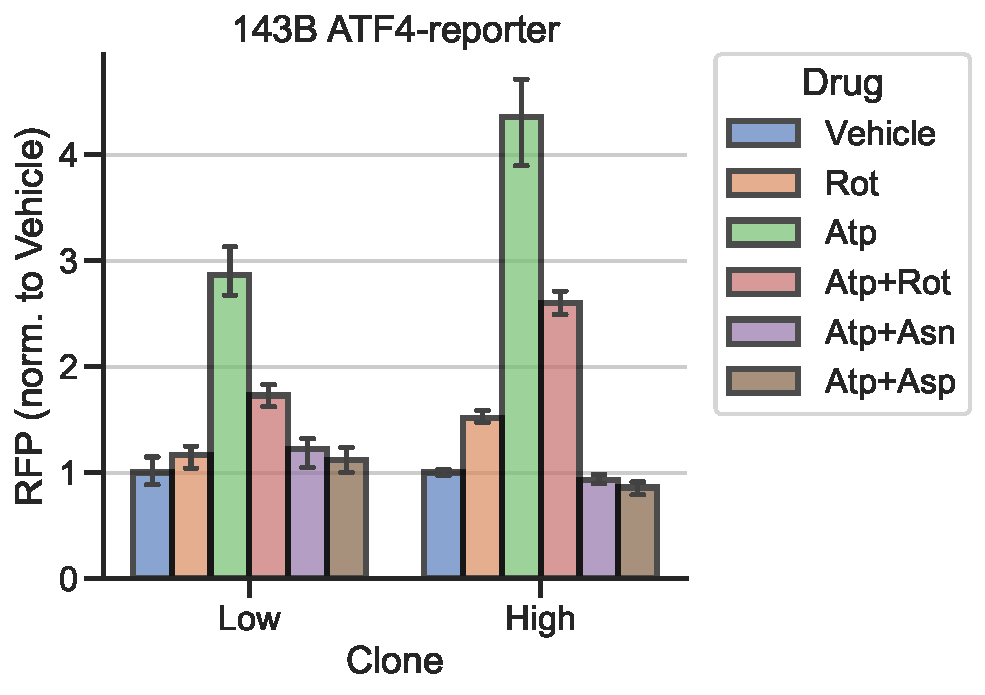
\includegraphics[width=\textwidth]{figures/chap2/143B_Atp_ATF4rep.pdf}
         \caption{ggg}
         \label{fig:ch2:143B_Atp_ATF4rep}
     \end{subfigure}
     \hfill
     \begin{subfigure}[b]{0.4\textwidth}
         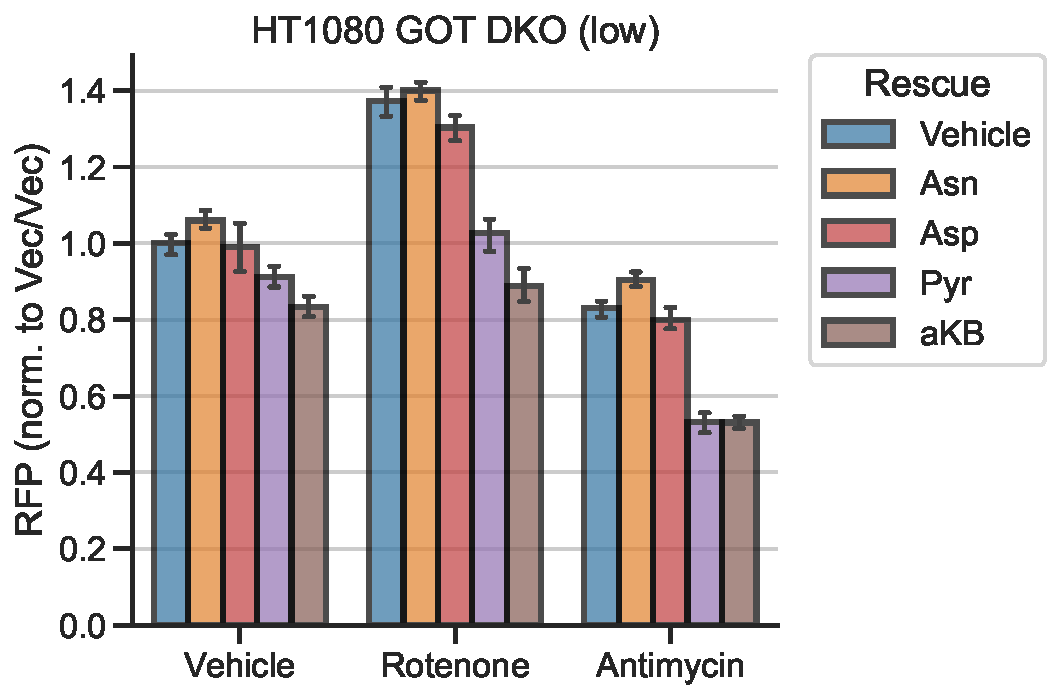
\includegraphics[width=\textwidth]{figures/chap2/HT1080_GOT_DKO_ETCinhib_ATF4rep.pdf}
         \caption{ggg}
         \label{fig:ch2:HT1080_GOT_DKO_ETCinhib_ATF4rep}
     \end{subfigure}
     \hfill
        \caption[ggg]{
        gggg
        }
        \label{fig:ch2:ISR}
\end{figure}











\section{Methods and Materials}

\subsection{Cell culture}
Cell lines were acquired from ATCC (143B, H1299, HT1080) and tested to be free from mycoplasma (MycoProbe, R\&D Systems).
Cells were maintained in Dulbecco’s Modified Eagle’s Medium (DMEM) (Gibco, 50-003-PB) supplemented with 3.7 g/L sodium bicarbonate (Sigma, S6297), 10\% fetal bovine serum (FBS) (Gibco, 26140079) and 1\% penicillin-streptomycin solution (Sigma, P4333).
Cells were incubated in a humidified incubator at 37°C with 5\% CO2.


\subsection{Western blots}
Protein lysates were harvested in RIPA buffer (Sigma, R0278) supplemented with Halt protease and phosphatase inhibitor cocktail (Fisher, PI78443) and 5 mM EDTA.
Protein concentration was determined using a bicinchoninic acid assay (Fisher, 23225) using bovine serum albumin (BSA) as a protein standard.
Equal amounts of protein were added to LDS sample buffer (ThermoFisher, B0008) and 5\% 2-Mercaptoethanol (Sigma, M3148), denatured at 95°C for 5 min, loaded onto 4–12\% SDS-polyacrylamide gels (Invitrogen, NW04122BOX) along with a prestained protein ladder (ThermoFisher, 26616) and run 35 min at 180V in MES buffer (ThermoFisher, B000202).
Proteins were dry transferred onto a 0.22 mm nitrocellulose membranes using the iBlot2 device (ThermoFisher, IB21001) with the P0 system setting and associated transfer stacks (Fisher, IB23001).
Membranes were blocked with 5\% bovine serum albumin; Sigma, A4503 in tris-buffered saline with 0.1\% Tween-20 (TBS-T) and incubated at 4°C overnight with the following antibodies:
anti-ATF4 (Cell Signaling, 11815S, 1:500),
anti-ASNS (Cell Signaling, 92479T, 1:1000),
anti-Phospho-eIF2alpha (Cell Signaling, 3398S, 1:500),
anti-eIF2alpha (Cell Signaling, 5324S, 1:500),
anti-Phospho-GCN2 (Cell Signaling, 94668S, 1:500),
anti-GCN2 (Cell Signaling, 3302S, 1:500),
anti-OMA1 (Cell Signaling, 95473, 1:1000),
anti-GADD34 (Proteintech, 10449-1-AP, 1:500),
anti-DARS2 (Proteintech, 13807-1-AP, 1:500),
anti-HRI (Sigma, HPA016496, 1:1000),
anti-FLAG (Sigma, F1804; 1:1000),
anti-SLC1A3 (Genetex, GTX20262; 1:500),
anti-GOT2 (Proteintech, 14800–1-AP, 1:750),
anti-GOT1 (Cell Signaling, 34423 S, 1:1000),
anti-Vinculin (Sigma, SAB4200729; 1:10,000) and anti-Tubulin (Sigma, T6199; 1:10,000).
Membranes were washed with TBS-T and the following secondary antibodies were added in blocking buffer: 800CW Goat anti-Mouse IgG (LiCOR, 926–32210; 1:15,000), 680RD Goat anti-Rabbit IgG (LiCOR, 926–68071; 1:15,000) and incubated for 1 hour.
Membranes were washed with TBS-T, incubated for 10 min in TBS-T, washed in deionized water and imaged on a LiCOR Odyssey Near-Infrared imaging system.


\subsection{Proliferation assays}
Cells were trypsinized (Corning, 25,051 CI), resuspended in seeding media, counted (Beckman Coulter Counter Multisizer 4) and seeded overnight onto 6/12/24-well dishes (Corning, 3516;3513:3524) with an initial seeding density of 10,000 cells/mL and a volume of 4, 2 and 1 mL, respectively.
After overnight incubation, 3–6 wells were counted for a starting cell count at the time of treatment.
Treatment was initiated either by media switch or by spike-in of drug/metabolite from a 20-50x stock.
Experiments were conducted in (both for seeding and treatment) DMEM without pyruvate (Corning 50–013-PB) supplemented with 3.7 g/L sodium bicarbonate 10\% dialyzed fetal bovine serum (FBS) (Sigma, F0392) and 1\% penicillin-streptomycin solution, with or without sodium pyruvate (Pyr) (Sigma, P8574),
2-ketobutyric acid (AKB) (Sigma, K401),
aspartate (Asp) (Sigma, A7219),
asparagine (Asn) (Sigma, A7094),
uridine (Urd) (Sigma, U3003), hypoxanthine (Cayman Chemical, 22254),
adenine (Ade) (Sigma, A2786),
guanine (Gua) (Sigma, 51030) or sodium formate (Sigma, 71539) with concentration noted when relevant.
Drug treatments included rotenone (Sigma, R8875),
metformin (Sigma, D150959),
atpenin A5 (Cayman Chemical, 11898; AdipoGen, AG-CN2-0110; Abcam, ab144194; or Enzo Life Sciences, ALX-380–313),
doxycycline hydrochloride (Sigma, D3447),
antimycin A (Sigma, A8674),
oligomycin A (Sigma, 495455),
GCN2iB (MedChemExpress, HY-112654),
FCCP (Cayman Chemical, 15218-10),
BAM15 (Cayman Chemical, 17811),
UCPH (HelloBio, HB0630) and DMSO vehicle (Sigma, D2650).
Cells were incubated in a humidified incubator at 37°C with 5\% CO2, then counted after 4–6 days.
Proliferation rate was reported as doublings per day and determined using the time and fold count difference between the starting and final counts and assuming a constant proliferation rate throughout the assay.


\subsection{Generation of nuclear RFP cell lines}
Nuclear RFP cell lines were generated using 1e5 transducing units of EF1A-nuclear RFP lentivirus (Cellomics Technology, PLV-10205-50) by spinfection.
Cells were seeded at 50\% confluency on 6 well dishes, lentivirus was added to fresh media with 8 µg/µL polybrene, then added to cells and followed by centrifugation (900g, 90 mins, 30°C).
Two days after infection, cells were sorted for high RFP expression using fluorescence-activated cell sorting (FACS).
High RFP cells were then expanded and single-cell cloned by limiting dilution, plating 0.5 cells/well on a 96 well plate.
Plates were then screened for RFP expression and localization using Incucyte S3 (Sartorius) and a suitable clone chosen, expanded, and used for all subsequent experiments.


\subsection{Incucyte measurements}
Proliferation assay using Incucyte



\subsection{Lentiviral production and stable cell line generation}
The following plasmids were obtained: pLenti6.3-V5 DEST\_SLC1A3 (DNASU Plasmid Repository), ATF4 reporter pXG237 (Addgene, 141281), pLHCX-gpASNase1 (Addgene, 121526) and pDONR221\_EGFP (Addgene, 25899).
ASNS was cloned by PCR from HEK293T reverse transcribed mRNA.
Genes were first cloned into entry vector pENTR1A (Fisher, A10462) using NEBuilder HiFI DNA Assembly Cloning Kit (New England BioLabs, E2621).
These donor constructs were then used to transfer their insert into destination vectors: pLX304-CMV-Blast (Addgene, 25890) or pLenti-CMV-Hygro (w117-1) (Addgene, 17454 a gift from Eric Campeau \& Paul Kaufman) using LR Clonase II (Fisher, 11791100).
Each plasmid sequence was verified by whole plasmid sequencing (Plasmidsaurus).
Lentivirus was generated by co-transfection of HEK293T cells with destination vector plasmid DNA and the packaging plasmids pMDLg/pRRE (Addgene, 12251), pRSV-Rev, (Addgene, 12253) and pMD2.G (Addgene, 12259) using FuGENE transfection reagent (Fisher, PRE2693) in DMEM (Fisher, MT10017CV) without FBS or penicillin-streptomycin.
The supernatant containing lentiviral particles was filtered through a 0.45 µM membrane (Fisher, 9720514) and was supplemented with 8 µg/µL polybrene (Sigma, TR-1003-G) prior to infection.
For infection, cells were seeded at 50\% confluency in 6 well dishes and centrifuged with lentivirus (900g, 90 mins, 30°C).
After 24 hours the media was replaced with fresh media and after 48 hours cells were treated with either 1 µg/mL blasticidin (Fisher, R21001) or 150 µg/mL hygromycin (Sigma, H7772-1G) and maintained in selection media until all uninfected control cells died.
After selection, cells were expanded and single-cell cloned by limiting dilution, plating 0.5 cells/well using 96 well plates.
These clones were expanded and screened by either western blot or presence of GFP or RFP signal using Incucyte S3 (Sartorius) to validate expression.
From this a single clone was chosen, expanded and used for all subsequent experiments.


\subsection{Generation of knockout cells}
Protocol and guide RNA generation was identical to that described in Hart et al. \cite{Hart2023-gp}.
Briefly, three chemically synthesized 2'-O-methyl 3’phosphorothioate-modified single guide RNA (sgRNA) sequences targeting the gene of interest were purchased (Synthego; table \ref{tab:ch2:guides}).
A pool of all three sgRNAs (or all six for GOT1/GOT2 double knockout) were resuspended in nuclease-free water, combined with SF buffer (Lonza, V4XC-2032), and sNLS-spCas9 (Aldevron, 9212).
200,000 H1299 cells were resuspended in the resulting solution containing ribonucleoprotein complexes (RNPs) and electroporated using a 4D-Nucleofector (Amaxa, Lonza).
Nucleofected cells were then expanded and single-cell cloned by limiting dilution by plating 0.5 cells/well in a 96 well plate.
Gene knockout was confirmed using western blots.

\begin{spacing}{1}
\begin{table}[ht]
\caption{\label{tab:ch2:guides}CRISPR guides.}
\begin{tabular}{|l|l|}
\hline
Gene & sgRNA   sequence (5’-3’) \\
\hline
GOT1 & \begin{tabular}[c]{@{}l@{}}\texttt{CAGUCAUCCGUGCGAUAUGC}\\\texttt{GCACGGAUGACUGCCAUCCC}\\\texttt{CGAUCUUCUCCAUCUGGGAA}\end{tabular} \\
\hline
GOT2 & \begin{tabular}[c]{@{}l@{}}\texttt{UUUCUCAUUUCAGCUCCUGG}\\\texttt{CGGACGCUAGGCAGAACGUA}\\\texttt{UCCUUCCACUGUUCCGGACG}\end{tabular} \\
\hline
OMA1 & \begin{tabular}[c]{@{}l@{}}\texttt{ACACAUUAGCAUCCACCUCA}\\\texttt{GAGUAAAUCAGUGUGACAGG}\\\texttt{GCCAACCCAAGAUGCCAGAA}\end{tabular} \\
\hline
HRI & \begin{tabular}[c]{@{}l@{}}\texttt{GUUUGCAACUGCAAAAGGGA}\\\texttt{UGAUGUUCCAGCAGAAAUCC}\\\texttt{CCAGCACCUUCACUUCCCGU}\end{tabular} \\
\hline
GCN2 & \begin{tabular}[c]{@{}l@{}}\texttt{AAAACUAAAUUGAUUUCAGG}\\\texttt{AGCUCGGUCAUCCUUGGCCA}\\\texttt{GAACUGGCCAAGAAACACUG}\end{tabular} \\
\hline
SLC25A10 & \begin{tabular}[c]{@{}l@{}}\texttt{GCAUCUGCAGACGCAGCAGG}\\\texttt{GCAACACCUUCUCGUGGAAG}\\\texttt{GAAGCUGCGCAUGACGGGCA}\end{tabular} \\
\hline
DARS2 & \begin{tabular}[c]{@{}l@{}}\texttt{ACAUAAAAUCUUCUUCACAG}\\\texttt{UGGUUAAGUCAGCUGUACAG}\\\texttt{GUGGAUGGAUUCAGUACCGA}\end{tabular} \\
\hline
\end{tabular}
\end{table}
\end{spacing}

\subsection{Polar metabolite extraction}
For polar metabolite extraction, a plate was move to ice and the media was thoroughly aspirated.
Wells were washed thrice with cold saline (Fisher, 23293184), 1 mL 80\% HPLC grade methanol in HPLC grade water was added, cells were scraped with the back of a P1000 pipet tip and transferred to Eppendorf tubes.
Tubes were centrifuged (17,000g, 15 mins, 4°C) and a fraction of the supernatant containing polar metabolites was transferred to a new centrifuge tube and placed in a centrivap until dry.
The fraction of supernatant transferred was adjusted to correspond to that extracted from a 1 µL cell volume e.g. 50\% was transferred if the total cell volume extracted from was 2 µL.
The total cell volume extracted from was determined by counting cells on a parallel plate using a coulter counter.
Dried samples were reconstituted with 40 µL 80\% HPLC grade methanol, containing internal standards if appropriate, and transferred to vials for measurement by LCMS.

\subsection{Media metabolite extraction}
For media metabolite extraction, 10 µL media was sampled, added to 990 µL 80\% HPLC grade methanol in HPLC grade water and incubated at -20°C for 30 min or until ready.
Tubes were centrifuged (17,000g, 15 mins, 4°C) and 400 µL of the supernatant containing media metabolites was transferred to a new centrifuge tube and placed in a centrivap until dry.
Dried samples were reconstituted with 40 µL 80\% HPLC grade methanol, containing internal standards if appropriate, and transferred to vials for measurement by LCMS.


\subsection{Absolute quantification by isotope dilution}
Dried samples were reconstituted with 40 µL 80\% HPLC grade methanol containing 5 µM U-\hCi, U-\hNi{} labelled canonical amino acid mix (Cambridge Isotope Laboratories, MSK-CAA-1) and transferred to vials for measurement by LCMS.
For pyrimidine nucleobase/nucleoside quantification a U-\hCi{} internal standard was made by partial hydrolysis (12 h in 6 M HCl at 90°C) of U-\hCi{} spirulina whole cells lyophilized powder (Cambridge Isotope Laboratories, CLM-8400-PK).
The peak area for each compound was divided by its labelled standard to derive the response ratio.
The response ratio was then mapped to a calibration curve to infer the compound concentration in the vial.
The sample concentration was calculated by correcting for each step introducing a dilution, for the intracellular concentrations this included using of the total cell volume.
To make the calibration curves a non-labelled amino acid mixture was made from an analytical amino acid standard without glutamine and asparagine (Sigma, A9906-1ML) and added glutamine (Sigma, 76523-100MG) and asparagine (Sigma, 51363-100MG) to match the concentration of the other amino acids.
For pyrimidine nucleobase/nucleoside quantification this pool was also mixed with equimolar uracil (Sigma, U1128), uridine (Sigma, U3003), 2′-deoxyuridine (Sigma, D5412), thymine (Sigma, T0376), cytosine (Sigma, C3506) and cytidine (Cayman Chemical, 29602).
Using this mix, three replicates of a 12 point 2-fold dilution series was made with a max concentration of 500 µM and a volume per dilution of 40 µL.
These were placed in a centrivap until dry and reconstituted with 40 µL 80\% HPLC grade methanol containing the appropriate isotopic internal standard and transferred to vials for measurement by LCMS.
The peak area for each compound was divided by its labelled standard to derive the response ratio, then the best fitting calibration curves for each compound were chosen among either linear, power or a second-degree polynomial.
Each calibration curve was manually inspected for proper fit and measurements below or above the concentration range of the dilution series were discarded.


\subsection{Liquid Chromatography-Mass Spectrometry (LCMS)}
Metabolite quantitation was performed using a Q Exactive HF-X Hybrid Quadrupole-Orbitrap Mass Spectrometer equipped with an Ion Max API source and H-ESI II probe, coupled to a Vanquish Flex Binary UHPLC system (Thermo Scientific).
Mass calibrations were completed at a minimum of every 5 days in both the positive and negative polarity modes using LTQ Velos ESI Calibration Solution (Pierce).
Polar Samples were chromatographically separated by injecting a sample volume of 1 µL into a SeQuant ZIC-pHILIC Polymeric column (2.1 x 150 mm 5 mM, EMD Millipore).
The flow rate was set to 150 mL/min, autosampler temperature set to 10°C, and column temperature set to 30°C.
Mobile Phase A consisted of 20 mM ammonium carbonate and 0.1\% (v/v) ammonium hydroxide, and Mobile Phase B consisted of 100\% acetonitrile.
The sample was gradient eluted (\%B) from the column as follows: 0-20 min.: linear gradient from 85\% to 20\% B; 20-24 min.: hold at 20\% B; 24-24.5 min.: linear gradient from 20\% to 85\% B; 24.5 min.-end: hold at 85\% B until equilibrated with ten column volumes.
Mobile Phase was directed into the ion source with the following parameters: sheath gas = 45, auxiliary gas = 15, sweep gas = 2, spray voltage = 2.9 kV in the negative mode or 3.5 kV in the positive mode, capillary temperature = 300°C, RF level = 40\%, auxiliary gas heater temperature = 325°C.
Mass detection was conducted with a resolution of 240,000 in full scan mode, with an AGC target of 3,000,000 and maximum injection time of 250 msec.
Metabolites were detected over a mass range of 70-850 m/z.
Quantitation of all metabolites was performed using Tracefinder 4.1 (Thermo Scientific) referencing an in-house metabolite standards library using ≤5 ppm mass error.
For samples subjected to stable isotope tracing, peak areas were natural abundance corrected with IsoCor \cite{Millard2019-hv}, using experimentally determined tracer purity values.



\subsection{Media uptake flux}
The cells were first passaged in DMEM with dialyzed FBS and the tracer and/or metabolites used during the uptake experiment.
For 143B GOT DKO cells expressing SLC1A3, 500 µM sodium aspartate was added to adjust intracellular aspartate levels.
For 143B WT cells, 100 µM U-\hCi{} Asn was added to achieve a steady-state label fraction in the proteome.
To start the experiment, cells were seeded on six well dishes at 1e5 cells/well.
On the next day fresh media was added and t=0 media samples were collected.
Then cells were incubated and subsequent media samples collected.
After the last media collection the residual media volume was quantified to correct for evaporation
For U-\hCi{} Asn tracing the labelling ratio was determined by extracting intracellular metabolites after the last media collection.
Two dishes were run in parallel and used for counting to determine proliferation rates and cell volume measurement using a coulter counter.

\subsubsection{Flux calculation}
Cell counts over time is assumed an exponential function ($y(t)$) with proliferation rate $K$ and cell count at $t=0$ being $y_0$:
\begin{equation}
    y(t) = y_0 2^{K t}
\end{equation}

Assuming amino acid uptake into a cell is constant, the uptake rate (also called influx) can be defined as the total molar uptake over a time range divided by the total area under the cell count curve of the same time range.
Formally, the flux of a compound $i$ is:
\begin{equation}
    F_i = \frac{n_i(t_1) - n_i(t_2)}{\int_{t_1}^{t_2} y(t) dt}
\end{equation}
With $F_i$ being the flux, $n_i(t)$ being the molar quantity of a compound $i$, and $t_1$ and $t_2$ being the first and second timepoint, respectively.

Using $\Delta$ to indicate the difference between $t_1$ and $t_2$, we can simplify the above:
\begin{equation}
    F_i = \frac{\Delta n_i}{\int_{t_1}^{t_2} y(t) dt} = \frac{\Delta n_i}{\frac{y_0 2^{K t_2}}{K\ \natlog(2)} - \frac{y_0 2^{K t_1}}{K\ \natlog(2)}} = \frac{\Delta n_i}{\frac{y_0 (2^{K t_2} - 2^{K t_1})}{K\ \natlog(2)}}
\end{equation}
The denominator is the area under the cell count curve from $t_1$ to $t_2$ and is sometimes referred to as ``cell hours'' because of its unit is time, typically hours.

Using cell hours it is possible to calculate the molar quantity taken up per cell per hour, typically as: $\frac{\text{fmol}}{\text{cell}\times h}$.
However, this makes it hard to compare across cell lines because of variability in cell size.
To fix this, simply redefine the problem from integrating the area under the cell count curve to the area under the cell volume curve.
The cell volume curve is defined using a volume per cell multiplier ($V_c$):
\begin{equation}
    V(t) = y(t) V_c = V_c y_0 2^{t K}
\end{equation}

Assuming cell volume is unchanged throughout the experiment, $V_c$ is a constant that is not integrated and we get:
\begin{equation}
    F_i = \frac{\Delta n_i}{\frac{V_c y_0 (2^{K t_2} - 2^{K t_1})}{K\ \natlog(2)}}
\label{eq:ch2:fl_vh}
\end{equation}
Since $V_c$ is a volume, we have a denominator with a typical unit of $\frac{L}{h}$.
We could call this ``volume hours'', and dividing a molar quantity onto this we typical get a unit of $\frac{\text{mM}}{h}$, which is comparable across cell lines with different sizes.

Sometimes it can be useful to convert the influx of a compound to its accumulated intracellular concentration, also referred to as total cell concentration.
The accumulated intracellular concentration of a compound can be understood intuitively as the total molar uptake divided by the total increase in cell volume.
To convert flux to total cell concentration for compound $i$ ($C_i$) observe the following rearrangement of equation \ref{eq:ch2:fl_vh}:
\begin{equation}
    F_i = K\ \natlog(2) \frac{\Delta n_i}{V_c y_0 (2^{K t_2} - 2^{K t_1})}
\end{equation}
The fraction is the total cell concentration for compound $i$ and thus we have:
\begin{equation}
    F_i = K\ \natlog(2) C_i => C_i = \frac{F_i}{K\ \natlog(2)}
\end{equation}


\subsubsection{Net asparagine consumption}
Human cells do not have any appreciable asparagine deaminase activity \cite{Sullivan2018-gz} and thus asparagine is a terminal metabolite that does not get converted or used as a substrate in other metabolic reactions.
This makes the asparagine fluxes suitable for isotope tracing if we make the explicit assumption is that asparagine can be generated from synthesis using aspartate but not recycled back.
Figure \ref{fig:ch2:asn_Jprot} shows the net asparagine fluxes when U-\hCi{} labelled Asn is added to the media.
Each net flux is the sum of fluxes in both directions e.g. U-\hCi{} Asn is net influxed because it is consumed while unlabelled Asn is net effluxed because it is absent from media at the initial conditions.

Influx and efflux can be measured by media sampling and using the ratio of labelled to unlabelled Asn inside the cell, the remaining fluxes can be solved.
Observe that the labelling ratio is defined by the influx, efflux and synthesis flux:
\begin{equation}
    \frac{\UAsn}{\Asn} = \frac{\Flin}{\Flsyn - \Flout}
\end{equation}

Isolate synthesis flux:
\begin{equation}
    \Flsyn = \frac{\Asn}{\UAsn} \Flin + \Flout
\label{eq:ch2:Jsyn}
\end{equation}

Introduce flux balance:
\begin{equation}
    \Flin + \Flsyn = \Flprot + \Flout => \Flprot = \Flin + (\Flsyn - \Flout)
\end{equation}

Isolate the flux of Asn deposition into protein ($\Flprot$) and insert $\Flsyn$ from equation \ref{eq:ch2:Jsyn}:
\begin{equation}
    \Flprot = \Flin + \left( \frac{\Asn}{\UAsn} \Flin + \Flout - \Flout \right)
\end{equation}

Simplify:
\begin{equation}
    \Flprot = \Flin \left( 1 + \frac{\Asn}{\UAsn} \right)
\label{eq:ch2:Jprot}
\end{equation}






\subsection{Acid hydrolysis}





Two 12W plates seeded in parallel (DMEM dia. FBS)
At 40-90\% confluency harvest by washing four times with saline
Count one plate
On the other plate add 1 mL 6M HCl to 5 wells, seal the plate and perform acid hydrolysis at 90C in incubator for 20h
Move hydrolysate to 2 mL tubes then wash the well thrice with 1 mL water and collect it in the same tube
Dry the hydrolysate
Add 0.5 mL 6M HCl to each tube and incubate another 48h at 90C, then dry
Reconstitute in 0.5 mL 6M HCl and aliquot 2 tubes with 10k cells and 2 tubes with 40k cells and dry.
Reconstitute the two 10k tubes with 1 mL water, move to a fresh tube, dry and reconstitute these with 40 uL SE+CAAv2 and run standard LCMS
Water reconstitution is an attempt to get rid of the plastic/glue soluble in HCl
Using uracil as a control (should be in the same range regardless of scraping or on plate hydrolysis)
% Sigma	84429-10X2ML	HCl for amino acid analysis






\subsection{Nitrogen-15 tracing}

\subsubsection{Salvage fraction of individual components}
The fractional contribution of individual components into their respective aspartate consuming fates was determined in 143B and H1299 cells for the salvageable metabolites asparagine (Asn), uridine (Urd), hypoxanthine (Hpx), adenine (Ade) and guanine (Gua) along with a vehicle treatment (Vec).
The salvageable metabolites were spiked-in from a 20x stock solution to achieve a final concentration of: 500 µM Asn, 200 µM Urd, 100 µM Hpx, 100 µM Ade or 100 µM Gua.
The fraction of salvage was determined by stable isotope tracing, performed using both Gln amide\=/\hNi{} (Cambridge Isotope Laboratories, NLM-557-PK) and Gln alpha\=/\hNi{} (Cambridge Isotope Laboratories, NLM-1016-PK) in separate reactions and added to DMEM without glucose, glutamine, pyruvate and phenol red (Sigma, D5030) supplemented with 10\% dialyzed FBS, 1\% penicillin-streptomycin, 25 mM glucose (Sigma, G7528).
The combination of cell lines, salvageable metabolites and tracers gave 2x6x2=24 conditions which were labelled to steady-state by culturing for four passages with a 1/20 split at each passage.
At the end of the last passage each condition was split into four technical replicates and plated on 24 well dishes (Corning, 3524).
Upon reaching confluency, polar metabolites were extracted and submitted to LCMS with the above described technique.

\subsubsection{Salvage fraction as a function of concentration}
Seeded H1299 and 143B cells at 5,000 and 10,000 cells/well on a 6-well dish in DMEM containing Gln amide\=/\hNi{} as described above.
Then added an equimolar mix of hypoxanthine and uridine from a 40x stock to a final concentration of 10, 20, 30, 40, 50, 60 µM in each of the 6 wells.
Fresh media was then added every four days and upon reaching confluency, polar metabolites were extracted and submitted to LCMS with the above described technique.








